% ----------- Cover Master Thesis Faculty of Sciences ---------------
% This document should be compiled with pdflatex.  If you want to use
% latex to compile to dvi/ps, you have to convert the images to (e)ps
%                           -- December 2012
% -------------------------------------------------------------------
\RequirePackage{fix-cm}
\documentclass[12pt,a4paper,oneside]{book}

% ------------------------- Load packages ---------------------------
% You can eventually add these while you load other packages
% in case you want to integrate the titlepage with the rest of your thesis
% -------------------------------------------------------------------
\usepackage{graphicx,xcolor,textpos}
\usepackage[english]{babel}
\usepackage{helvet}
\usepackage{amsmath}
\usepackage{mathtools}
\usepackage{textcomp}
\usepackage{multicol}
\usepackage[round]{natbib}
\usepackage{caption}
\usepackage{subcaption}
%\usepackage{todonotes}
%\usepackage{hyperref}

% ------------------------ Page settings -----------------------------
% If you change these, the cover layout will also change.  In that
% case you have to adjust the latter manually.
% --------------------------------------------------------------------

\topmargin -10mm
\textwidth 160truemm
\textheight 240truemm
\oddsidemargin 0mm
\evensidemargin 0mm

% ---------------------- textpos settings ----------------------------
% Some additional settings for the cover
% --------------------------------------------------------------------

\definecolor{green}{RGB}{172,196,0}
\definecolor{bluetitle}{RGB}{29,141,176}
\definecolor{blueaff}{RGB}{0,0,128}
\definecolor{blueline}{RGB}{82,189,236}
\setlength{\TPHorizModule}{1mm}
\setlength{\TPVertModule}{1mm}

\begin{document}

% ----------------------- Cover --------------------------------------
% Please fill in:
% - The title and subtitle (if applicable)
%         to include a formula in the title or subtitle
%         use  \form{$...$}
% - Your name
% - Your (co)supervisor, mentor (if applicable)
% - Your master
% - The academic year
% --------------------------------------------------------------------
\thispagestyle{empty}
\newcommand{\form}[1]{\scalebox{1.087}{\boldmath{#1}}}
\sffamily
%
\begin{textblock}{191}(-24,-11)
\colorbox{green}{\hspace{139mm}\ \parbox[c][18truemm]{52mm}{\textcolor{white}{FACULTY OF SCIENCE}}}
\end{textblock}
%
\begin{textblock}{70}(-18,-19)
\textblockcolour{}
\includegraphics*[height=19.8truemm]{LogoKULeuven}
\end{textblock}
%
\begin{textblock}{160}(-6,63)
\textblockcolour{}
\vspace{-\parskip}
\flushleft
\fontsize{40}{42}\selectfont \textcolor{bluetitle}{Radiation-Hydrodynamics with MPI-AMVRAC: Massive-Star Atmospheres and Winds}\\[1.5mm]
\fontsize{20}{22}\selectfont CAK-theory and flux limited diffusion
\end{textblock}
%
%\begin{textblock}{82}(50,103)
%\textblockcolour{}
%\vspace{-\parskip}
%\flushleft
%\fbox{\parbox{79mm}{The background can be left blank or you can insert an image (maximum height 10 cm, width variable, mind author’s rights…). NO logos (you can use the logos inside the manuscript, but not on front or back cover). \textit{Delete this textbox.}}}
%\end{textblock}
%
\begin{textblock}{160}(8,153)
\textblockcolour{}
\vspace{-\parskip}
\flushright
\fontsize{14}{16}\selectfont \textbf{Nicolas MOENS}
\end{textblock}
%
\begin{textblock}{70}(-6,191)
\textblockcolour{}
\vspace{-\parskip}
\flushleft
Supervisor: Prof. J. Sundqvist\\[-2pt]
\textcolor{blueaff}{KULeuven \textsl{(IVS)}}\\[5pt]
Co-supervisor: Dr. I. El Mellah\\[-2pt]
\textcolor{blueaff}{KULeuven \textsl{(CMPA)}}\\[5pt]
\end{textblock}
%
\begin{textblock}{160}(8,191)
\textblockcolour{}
\vspace{-\parskip}
\flushright
Thesis presented in\\[4.5pt]
fulfillment of the requirements\\[4.5pt]
for the degree of Master of Science\\[4.5pt]
in Astronomy and Astrophysics\\
\end{textblock}
%
\begin{textblock}{160}(8,232)
\textblockcolour{}
\vspace{-\parskip}
\flushright
Academic year 2017-2018
\end{textblock}
%
\begin{textblock}{191}(-24,248)
{\color{blueline}\rule{550pt}{5.5pt}}
\end{textblock}
%
\vfill
\newpage

\begin{textblock}{160}(-6,191)
\textblockcolour{}
\center
\thispagestyle{empty}

\textcopyright Copyright by KU Leuven

Without written permission of the promotors and the authors it is forbidden to reproduce or adapt in any form or by any means any part of this publication. Requests for obtaining the right to reproduce or utilize parts of this publication should be addressed to KU Leuven, Faculteit Wetenschappen, Geel Huis, Kasteelpark Arenberg 11 bus 2100, 3001 Leuven (Heverlee), Telephone +32 16 32 14 01.

A written permission of the promotor is also required to use the methods, products, schematics and programs described in this work for industrial or commercial use, and for submitting this publication in scientific contests.
\vfill
\end{textblock}
\newpage

% In case you want to integrate the TeX-file for the titlepage
% with the rest of your thesis, you cab continue below
% ------------------------- First pages ---------------------------
% For table of contents, acknowlegments, ...
% -----------------------------------------------------------------
\rmfamily
\setcounter{page}{0}
\pagenumbering{roman}

\chapter*{Preface}
Thank you everybody
\chapter*{Summary}
Something something modeling stellar winds
\chapter*{Summary in layman's terms}
Most matter in the universe is not gaseous, liquid or solid. Most matter in the universe is in a fourth state: plasma, ionised gas. Stars, nebulae and some interstellar clouds all consist of this state of matter. Modelling the movement of plasmas is done with sophisticated computer codes, as its behaviour can be very chaotic. Another important player in the universe is radiation. Most objects we see in the skies, the sun during the day and the stars during the night are emitting strong electromagnetic fields.\\

As you may know, matter and radiation can interact. Not only can radiation heat materials (that's why it is warm when the sun is out), objects also cool when they emit themselves, and radiation can exert a force on an object: think about solar sails being used on satellites. In many astrophysical contexts this interaction is of great importance. For example: the most massive stars blow away parts of their outer layers due to this radiation force; The temperature of objects surrounding stars is set by the stellar radiation field like the temperature on earth is set by the sun.\\

This thesis focusses on adapting a computer code used to model plasmas and add a parts to it which describe the interaction between radiation and plasma. After writing the code, of course it has to be tested to check if everything works. The end product is not only a working and tested computer code, time was also spent on modelling the matter being blown away from stellar surfaces and the insides of a star.  

%\thispagestyle{empty}
\chapter*{List of abbreviations and symbols}
\begin{multicols}{2}
\section*{Abbreviations}
\begin{tabular}{ll}
HD     & Hydrodynamics             \\
RHD    & Radiohydrodynamics        \\
LTE    & local thermal equilibrium \\
CAK    & Castor, Abott and Klein   \\
FLD    & Flux limited diffusion    \\
MPI    & message passing interface \\
AMR    & adaptive mesh refinement  \\
VAC    & versatile advection code  \\
PDE    & partial differential equations \\
BH     & black hole \\
NS     & neutron star \\
WD 	   & white dwarf \\
\end{tabular}

\section*{General}
\begin{tabular}{ll}
$c$               & speed of light \\
$M_\odot$         & solar mass  \\
$R_\odot$         & solar radius\\
$L_\odot$         & solar luminosity \\

\end{tabular}

\section*{Hydrodynamics}
\begin{tabular}{ll}
$\rho$         & density       \\
$\vec{v}$      & velocity      \\
$e$		  	   & gas energy density   \\
$p$		  	   & gas pressure  \\
$\gamma$       & adiabatic index \\
$a_{adiab}$    & adiabatic soundspeed \\
$T$		  	   & gas temperature \\
$\nabla$       & gradient\\
$\vec{\nabla}$ & divergent\\
$S_{\rho, \vec{v}, e}$ & sourceterms for HD-equations\\
$g_{grav}$     & gravitational acceleration \\
$g_{rad}$	   & radiative acceleration \\
\end{tabular}


\section*{Radiation hydrodynamics}
\begin{tabular}{ll}
$\Gamma$      & Eddington factor \\
$\nu$         & frequency \\
$\Omega$      & solid angle \\
$\kappa_\nu$  & opacity at frequency $\nu$ \\
$\kappa$      & Rosseland mean opacity\\
$\chi_\nu$    & absorption coefficient at frequency $\nu$ \\
$\eta_\nu$    & emission coefficient at frequency $\nu$ \\
$\vec{n}$     & unit vector along line of sight\\
$S_\nu$       & source function\\
$B_\nu$       & Planck function\\
$I_\nu$, $I$  & frequency dependent and integrated intensity\\
$J_\nu$, $J$  & mean intensity\\
$E_\nu$, $E$  & radiation energy density\\
$\vec{F}_\nu$,$\vec{F}$ & radiation flux\\
$H_\nu$, $H$  & $1^{st}$ moment of intensity\\
$P_\nu$, $P$  & radiation pressure\\
$K_\nu$, $K$  & $2^{nd}$ moment of intensity \\
%%%%%%%%%%%%%%%%%%%%%%%%%%%%%%%%%%%%%%%%%%%%%%%%%%%%%
$H_{eff}$     & scale height \\
$g_{eff}$ 	  & effective acceleration \\
$\tau$        & optical depth \\
\end{tabular}

\section*{CAK and FLD}
\begin{tabular}{ll}
$l_{sob}$          & sobolev length \\
$g_{line}$         & line acceleration\\
$\kappa_e$         & electron opacity \\
$q$                &   \\
$t$                &   \\
%%%%%%%%%%%%%%%%%%%%%%%%%%%%%%%%%%%%%%%
$\lambda$          & flux limiter \\
$l_\gamma$		   & photon mean free path \\
$R$                & ratio of $l_\gamma$ and radiation scale height\\
$D$                & diffusion coefficient\\
\end{tabular}

\section*{Numerics}
\begin{tabular}{ll}
$\Delta x$       & cell width in the $x$-direction\\
$\Delta t, dt$	 & time step \\
$N,M$            & dimension of grid \\
$\tilde{x}$      & quantity $x$ in dimensionless units \\
$x_0$		     & the normalised value of quantity $x$ \\
$x_{i,j}^n$	     & quantity $x$ at timestep $n$ in cell $i,j$ \\
\end{tabular}


\end{multicols}

\listoffigures
\listoftables
\tableofcontents

\newpage
% -------------------------- Proper text --------------------------
% Introduction, chapters, ...
% -----------------------------------------------------------------
\setcounter{page}{0}
\pagenumbering{arabic}

\chapter{Introduction}
\section{Astrophysical context}
%General situation Astrophysics
High mass stars are the drivers of dynamical and chemical evolutions of galaxies throughout the Universe, including our own Milky Way. Massive stars live short but exciting lives, finally ending in giant supernova explosions. After their death they leave behind exotic remnants such as neutron stars (NS) or black holes (BH). Whether a massive star ends as either NS or BH depends a lot on the amounts of mass expelled during their lifetime due to stellar winds. Moreover, mass loss through high-mass stellar winds and atmospheres is critical to further understand the quite unexpected BH mass distribution observed by the LIGO collaboration \citep{TheLIGOScientificCollaboration2016}, \citep{Abbott1} trough gravitational waves, to which data is being added as we speak. BH's have been observed with masses of about $30$ times that of our sun, it's not quite sure which processes lead to these mass ranges.\\

%General importance radiative processes
In many astrophysical systems it is important to take into account a radiation field when considering gas dynamics (\citep{Tetsu2016},  ...). Radiation can exert forces to, for example, accelerate stellar winds and transport energy in non-convective stellar radiation zones. The equations describing gas dynamics with a radiation field will further evolve on two different timescales, a radiation field generally evolves much faster than gas, so solving the gas and radiation dynamics equations together is quite generally a very challenging task. \\

%Develop models
This thesis focusses developing new radiation modules to be used in the gerenral purpose numerical hydrodynamics code \texttt{MPI-AMRVAC}, developed in-house at KU-Leuven. Radiation has, except for a radiative cooling module, until now not been represented in this code. Two targeted first applications for these modules regard the stellar atmospheres and stellar wind outflows of very massive stars. So next to modelling stellar winds and atmospheres, a main result of this thesis are computer codes written to be used with \texttt{MPI-AMRVAC} which will be used in research on radiation dominated processes.\\

%More examples of radiation dominated processes
An important concept in these systems where radiation strongly affects it's dynamics is the Eddington factor $\Gamma$, this is the ratio between the radiative and gravitational acceleration.
\begin{align}
	\Gamma = \frac{\kappa F_r}{c g_{grav}}
\end{align}
Where $F_r$ is the radiation energy flux component parallel but in opposite direction to the gravitational field. $\kappa$ Is the absorption opacity in $[\frac{cm^2}{g}]$, $c$ the speed of light in vacuum and $g_{grav}$ the magnitude of the local gravitational acceleration. If the Eddington factor describing a system increases, the importance for taking into account radiation grows as well.The importance of good models for radiation hydrodynamics is clear in a multitude of astrophysical systems, a few are listed below. Quite generally, many of these systems are characterized by a high Eddington factor, possibly leading to for example radiation driven instabilities, structured density distributions and direct outflows. Here, a few typical radiation dominated regimes are given as an example:

\begin{itemize}
\item \textbf{stellar winds}\\
The basic requirement for driving a stellar wind is an outward pushing force, this force must be strong enough to be able to overcome the opposing gravity so that material can escape the star. Based on which type of opposing force is prevailing, winds can be subdivided in three types: \emph{pressure driven} for solar type stars, \emph{dust driven} for cool massive stars and \emph{radiation driven} for hot massive stars \citep{Lamers1999}. The driving force behind these radiation driven winds is, as the name suggests, radiation force. In other words, $\Gamma > 1$. Outwards travelling photons get absorbed or scattered by atomic line transitions and (some of) the photon's momentum is transferred to the ion or atom. Hot massive stars can undergo mass loss of $\sim 10^{-6} M_\odot/yr$ due to radiation driven winds, this of course will have an impact on their evolution.
%Stars with a luminosity of $10^6 L_\odot$ and a stellar mass of $80 M_\odot$ will have an Eddington factor $\Gamma \sim 50$ near the surface, radiation plays an essential role in their dynamics.
CAK-theory, (Castor Abbott and Klein) is an analytical model describing these winds, and the first half of this thesis was spent on modelling this.\\
Dust driven winds escape from cooler massive stars. They are also driven by radiation, however in contrast to the hot stellar radiative winds, the opacity source in the system is caused by the dust instead of atomic absorption lines or electron scattering. Pressure driven winds, like the one escaping our sun, are driven by the pressure gradient. Solar type stars have a higher pressure gradient as compared to massive stars due to their smaller pressure scale height. Also, the radiation field is orders of magnitude lower, and thus less radiation force is available to accelerate the gas. These winds are also studied at KU-Leuven, but will not be considered in this thesis.


\item \textbf{stellar atmospheres}\\
In stellar atmospheres like that of our sun, the radiation field is directly responsible for setting the temperature structure. Energy created by fusion processes in the stellar core is transported outward by the radiation field. The atmosphere is said to be in radiative equilibrium, this means that the radiation energy absorbed by the atmospheric gas is equal to the energy that is radiated. 

\item \textbf{stellar and galactic disks}\\
Accretion disks appear in all sorts of objects: young stellar objects, pre-main sequence objects, various types of stars, around BH's, NS's,  and on a much larget scale around active galactic nuclei (AGN) \citep{Proga2009} and so on. The gas in these disks is often heated due to internal collisions or accretion on the central object, which gives rise to a significant radiation field. This radiation field can highly impact the disk shape and energy distribution within the disk due to ablation and radiative heating \citep{Kee2018}, \citep{Nakatani2017}. \\
AGN disks also drive winds on the surface of their disks. Moreover, the conditions far away in AGN disks actually resemble those found at the surface of massive stars. These systems can also launch radiation driven disk winds \citep{Proga2009}.

\item \textbf{star formation}\\
During the collapse of interstellar gas clouds during the process of star formation, energy transport due to radiation has effects on the formation process of pre-stellar cores \citep{Bhandare2017}. A big open question in astrophysics is what physical mechanism sets the upper mass limit for in the formation of massive stars. One proposed mechanism is the accretion leading to a radiation field raising $\Gamma_e$ above unity. This provides a feedback loop that calls a halt to mass accretion \cite{Vink2018}.

%\item \textbf{very massive stars}\\

\item \textbf{interstellar medium}\\
The interstellar medium (ISM) is home to numerous types of gas clouds. A prominent example of a regime where radiation plays an important role are so called HII regions. These hydrogen clouds surrounding hot massive stars are ionised by the stellar UV-photons. Due to the radiative heating of the gas, these clouds are ever expanding. \citep{ISM course notes}, \citep{Klaassen2017}. 

\item \textbf{Eruptive variables}\\
Systems that exceed the Eddington limit ($\Gamma > 1$) even when only electron scattering is considered are called super-Eddington systems. A prime example for such a system is $\eta$ Carinae. $\eta$ Carinae is what is known as an eruptive variable. It is a star which underwent an enormous mass loss in the middle of the 19th century, losing $10 M_\odot$ over the course of $10$ years. One of the hypothesised drivers of this huge mass loss is radiation\citep{Smith2003}.
\end{itemize}

Methods used and codes developed in this project are applicable in a very broad range of scenarios. Having provided the reader with adequate potential uses for the numerical tools developed, this thesis describes radiation hydrodynamics (RHD) in two different regimes: CAK-theory in optically thin hot stellar winds and flux limited diffusion in optically thick stellar atmospheres. Before we move to the mathematical framework of radiative fluids, let us first have a short review of the equations describing gases and liquids.\\

\section{Hydrodynamics}
The movement of non-isothermal isotropic gases and fluids in the absence of magnetic fields and radiation, and no significant viscosity, can be described by ideal hydrodynamics. The hydrodynamical equations describe conservation of mass, conservation of momentum and conservation of energy in the following equations:

\begin{align}
 \partial_t \left(\rho \right) + \vec{\nabla} \cdot \left( \rho \vec{v}  \right) &= S_\rho \label{eq: hd_rho}\\
 \partial_t \left(\rho \vec{v} \right) + \vec{\nabla} \left( \vec{v} \rho \vec{v} + p \right) &= S_{\rho \vec{v}} \label{eq: hd_mom}\\
 \partial_t \left(e \right) + \vec{\nabla} \cdot \left( \vec{v} e + \vec{v} p \right) &= S_e \label{eq: hd_e}
\end{align}

These three partial differential equations (PDE's) are called the continuity equation (describing mass conservation \eqref{eq: hd_rho}), the momentum equation (describing momentum conservation \eqref{eq: hd_mom} ) and the energy equation (describing conservation of the total energy \eqref{eq: hd_e}). Above, the equations were written in their conservative form, they all have the same shape:

\begin{align}
	\partial_t \underbrace{u}_\text{density} + \vec{\nabla} \cdot \overbrace{\vec{f_u}}^\text{density flux} &= \underbrace{S_u}_\text{source term} \label{eq: conservative}
\end{align}

There are only three PDE's describing four primitive variables: mass density $\rho$, velocity $\vec{v}$, gas energy density $e$ and gas pressure $p$, $\rho \vec{v}$ is the momentum density. This means that there is need for an additional closure relation, an equation of state like for example the ideal gas law:
\begin{align}
	p = (\gamma - 1) \left(e - \frac{\rho \vec{v}^2}{2} \right) \label{gas_closing}
\end{align}
where $\gamma$ is the adiabatic index.\\

The source terms in the equations describe (external) additions or subtractions to one of the densities: $S_\rho$ describes mass being added or subtracted from the system, $S_{\rho \vec{v}}$ describes external forces such as gravity or radiative forces and $S_e$ describes work exerted on the system, this can be for example due to heating or cooling of the fluid by a radiation field. A good description of radiation hydrodynamics needs to formulate the correct source terms for the momentum equation \eqref{eq: hd_mom} and gas energy equation \eqref{eq: hd_e}. These source terms can depend on the other primitive variables $\rho$, $\vec{v}$ and $e$ as well as parameters describing the source of the radiation field such as the luminosity and mass of a central object (star, AGN, ...).\\

Predicting fluid dynamics means solving these aforementioned equations simultaneously. Some cases can be solved analytically after making some assumptions, but for most practical cases this is done using numerical computer codes such as \texttt{mpi-AMRVAC} \citep{Porth2014}. Solving these equations is a tricky business, and there are numerous codes and numerical schemes available. The evolution of a simulation will depend not only on both initial and boundary conditions, but also on which physics one takes into consideration (sourceterms) and even a little on which numerical methods are used, more on this in chapter \ref{section: methods amrvac}. \\

In section \ref{section: introduction CAK}, an analytic expression for the radiation force momentum source term is derived to simulate the conditions in line driven stellar winds. This analytical calculation was first done by Castor, Abbott and Klein \citep{CAK1975} and carries their initials in its name: CAK-theory. The following section will illustrate the derivation of a more general formalism for radiation caused source terms., not only for the momentum but also the energy equation. 

\section{Radiation Hydrodynamics}
The last section gave a small recap of hydrodynamics. In this section, a mathematical framework is set up to combine the hydrodynamics equations with the effects of a potentially time dependent radiation field. At the end of this we will be left with a system of partial differential equations describing the dynamics of both the gas and the radiation field.\\ 
The main governing equation describing the evolution of radiation through a medium is the radiative transfer equation:
\begin{align}
\left( \frac{1}{c} \frac{\partial}{\partial t} + \vec{n} \cdot \vec{\nabla} \right) I_\nu = \eta_\nu + \chi_\nu I_\nu \label{eq: RTE}
\end{align}
where $I_\nu$ is the intensity at frequency $\nu$ along the direction of unit vector $\vec{n}$. $\eta_\nu$ And $\chi_\nu$ are the emissivity and total opacity. This equation describes how the value of the intensity $I_\nu$ changes when propagating trough a medium with given emissivity and opacity. The literature can be a bit confusing when handling the opacity and the absorption coefficient. So to avoid any confusion: the absorption coefficient $\chi$, generally given in units of $\frac{1}{cm}$ is the product of the opacity $\kappa$ given in $\frac{cm^2}{g}$ and the density $\rho$.\\

%The $1^{st}$  order radiative transfer equations are obtained by integrating over all solid angles and dividing by $4 \pi$, the $2^{nd}$ order one by first multiplying with $\vec{n}$ before doing the integration.\\
The so-called moment equations of radiative transfer are obtained by integrating over all solid angles and dividing by $4 \pi$ for the first order moment equation, and for the $2^{nd}$ order one by first multiplying with $\vec{n}$ before doing the integration.\\

\begin{align}
\frac{1}{c} \frac{\partial J_\nu}{\partial t} + \vec{\nabla} \cdot \vec{H_\nu} &= \frac{1}{4 \pi} \int_\Omega \eta_\nu + \chi_\nu I_\nu d\Omega \\
\frac{1}{c} \frac{\partial \vec{H_\nu}}{\partial t} + \vec{\nabla} \cdot K_\nu &= \frac{1}{4 \pi} \int_\Omega \left( \eta_\nu + \chi_\nu I_\nu\right) \vec{n} d\Omega
\end{align}

Where $J_\nu$, $\vec{H_\nu}$ and $K_\nu$ are the higher order moments of the intensity. $J_\nu$ is the mean intensity, which is $I_\nu$ averaged over all solid angles, and thus a scalar. $\vec{H}_\nu$ Is a vector and $K_\nu$ is a tensor of order 2. The following relations exist between the moments of intensity and some more physical quantities:

\begin{align}
E_\nu &= \frac{4 \pi}{c} J_\nu = \frac{1}{c} \int_\Omega I_\nu d \Omega\\
\vec{F_\nu} &= \frac{4 \pi}{c} \vec{H_\nu} = \frac{1}{c} \int_\Omega I_\nu \vec{n} d \Omega\\
P_\nu &= \frac{4 \pi}{c} K_\nu = \frac{1}{c} \int_\Omega I_\nu \vec{n}\vec{n} d \Omega
\end{align}

These are the radiative energy $E_\nu$, the radiation flux $\vec{F_\nu}$, and the radiation pressure tensor $P_\nu$. When assuming an isotropic radiation field, just like with the gas pressure tensor, $P_\nu$ can be written as a scalar times the unit tensor. The fraction of emissivity and total opacity is often written as the source function $S_\nu = \frac{\eta_\nu}{\chi_\nu}$. \\
 When doing full radiative transfer, these equations are solved for an enormous amount of frequencies, corresponding to the indices $_\nu$. The situation is simplified when assuming a frequency independent absorption and emission. This simplifies the equations because the radiation quantities $(I_\nu, \vec{F}_\nu, E_\nu, ...)$ can now be integrated over all frequencies, dropping their index. The local thermal equilibrium (LTE), frequency integrated radiation energy and radiation flux equations can be written in a conservative form, similar to the hydrodynamics equations: 

\begin{align}
\frac{\partial E}{\partial t} + \vec{\nabla} \cdot \vec{F} &= \int_\Omega \chi_\nu \left( S + I \right) d\Omega \label{eq: E_si}\\
\frac{\partial \vec{F}}{\partial t} + c^2 \vec{\nabla} P &= \int_\Omega \chi \left( S + I \right) \vec{n} d\Omega \label{F_si}
\end{align}

Assuming LTE, the source function is equal to the Planck function $S_\nu = B_\nu(T)$ and both $B_\nu(T)$ and $\chi_\nu$ are independent of solid angle. The relations between flux, energy and the moments of intensity can be used again to replace $I_\nu$ in the source terms. Because of symmetry, $S_\nu \vec{n}$ integrated over the total solid angle will return $\vec{0}$ in the source term of the flux equation.\\

The absorption coefficient is the product of the gas density and the frequency dependent opacity: $\chi_\nu = \rho \kappa_\nu$. Integrating the left hand sides of equations \ref{eq: E_si} and \ref{eq: F_si} over solid angle, where the full integral over $J_\nu \vec{n} $ leads to:
\begin{align}
\frac{\partial E}{\partial t} + \vec{\nabla} \cdot \vec{F} &= 4\pi \kappa\rho B(T) - c \kappa \rho E\\
\frac{\partial \vec{F}}{\partial t} + c^2 \vec{\nabla} P &=  c \kappa \rho \vec{F} 
\end{align}

In a more general form, where the absorption an emission coefficient are not frequency independent, the frequency independent opacities should be replaced by suitable averages. An energy-averaged, Plack-averaged and flux-averaged opacity can be defined. In the static diffusion limit (see \ref{section: introduction Flux Limited Diffusion}) al these averaged opacities are equal. They are given by the Rosseland mean opacity:
\begin{align}
\frac{\int_\nu E_\nu \kappa_\nu d\nu}{\int_\nu E_\nu d\nu} = \frac{\int_\nu B_\nu \kappa_\nu d\nu}{\int_\nu B_\nu d\nu} = \kappa = \frac{\int_\nu \vec{F}_\nu \kappa_\nu d\nu}{\int_\nu \vec{F}_\nu d\nu}
\end{align}

These equations are written here in the static observer's frame. Transforming them to a co-moving frame, the same frame as used in aforementioned hydro equations, is done in \citep{Mihalas1984a} by complicated Lorentz transformations. Effectively an advection term is added to the density flux in  both equations: $\vec{v} E$ and $\vec{v} \cdot \vec{F}$. The two source terms in the radiation energy equation are interpreted as energy exchange between the gas and the radiation field: energy leaving the radiation field heats the gas and gas is cooled by energy entering the radiation field. These so called heating and cooling source terms, $4\pi \kappa\rho B(T)$ and $ c \kappa \rho E$, must be added to the gas energy equation as well. In a steady state radiative equilibrium regime ($S = B = J = \frac{c}{4\pi}E$), these terms cancel each other out.\\

Another source term in the radiative energy equation that needs to be added is the photon tiring term $\vec{\nabla} \cdot \vec{v} P $. This term expresses the work done by the photons in the radiation field to accelerate the gas. It is essentially the radiation energy equivalent of the momentum radiation force term. The origin of this term is also explained more carefully in \citep{Mihalas1984a}. \\

The source term in the radiation flux equation has the same units as the gas momentum source term, this is the expression for radiation force. If momentum leaves the radiation flux, there is work being done. This must also mean that there is energy leaving the radiation field. That energy loss is translated in the photon tiring term $\vec{\nabla} \cdot \vec{v} P$, which must be subtracted from the radiation energy source term. The final system of PDE's read:

\begin{align}
 \partial_t \left(\rho \right) + \vec{\nabla} \cdot \left( \rho \vec{v}  \right) &= 0 \label{eq: rhd_cont} \\
 \partial_t \left(\rho \vec{v} \right) + \vec{\nabla} \left( \vec{v} \rho \vec{v} + p \right) 
 &= \frac{\kappa \rho}{c} \vec{F} \label{eq: rhd_mom} \\
 \partial_t \left(e \right) + \vec{\nabla} \cdot \left( \vec{v} e + \vec{v} p \right) &= -4\pi \kappa\rho B + c \kappa \rho E \label{eq: rhd_e}\\
 \partial_t \left(E \right) +  \vec{\nabla} \cdot \left( \vec{v} E + \vec{F} \right) &=  -\vec{\nabla} \cdot \vec{v} P + 4\pi \kappa\rho B - c \kappa \rho E \label{eq: rhd_e_r} \\
 \partial_t \left(\frac{\vec{F}}{c^2} \right) +  \vec{\nabla} \left( \frac{\vec{v} \cdot \vec{F}}{c^2} + P \right) &= - \frac{\kappa \rho}{c} \vec{F} \label{eq: rhd_flux}
\end{align}

These are the final radiation hydrodynamics equations. There are only 5 equations for 7 primitive variables: $\rho$, $\vec{v}$, $e$, $p$, $E$, $\vec{F}$ and $P$. Two closing relations are necessary to close the system. A first closing relation is obtained by re-using the ideal gas law \eqref{gas_closing}, a second one can be obtained by for example the \emph{Flux limited diffusion} approximation (FLD) described in section \ref{section: introduction Flux Limited Diffusion}.

\section{Sobolev and CAK-theory} \label{section: introduction CAK}
CAK-theory is a formalism developed by Castor, Abbot and Klein \citep{CAK1975} describing the radiative acceleration of the gas $g_{rad} = \frac{\kappa F}{c}$. Gas is accelerated in the line of sight of a radiation source, an ensemble of scattering and absorption lines leads to a significant radiative acceleration. The theory can be applied in the radiation driven winds of for example hot massive stars and in disk winds from active galactic nuclei. Let's begin here by writing down the acceleration caused by free electron scattering. Consider a star with mass $M_*$ and luminosity $L_*$. If only electron scattering is assumed, light gets absorbed and re-emitted equally. If $\kappa_e$ is defined as the electron scattering opacity, the radiative acceleration at any radial distance r is given by:
\begin{align}
g_e = \frac{\kappa_e L_*}{4 \pi r^2 c}
\end{align}
The gravitational attraction of the gas is given by Newtons gravitation law and is equal to $g_{grav} = G\frac{M_*}{r^2}$. Both accelerations vary as $\frac{1}{r^2}$, so their ratio is constant as a function of radius. An Eddington parameter for a purely electron scattering radiation force is defined as $\Gamma_e$:
\begin{align}
\Gamma_e = \frac{\kappa_e L_*}{4 \pi G M_* c}
\end{align}
Let's now have a look at radiative acceleration of a single absorption line in a line driven wind. Consider a set of ions absorbing at $\lambda_0$. These ions have very high velocities and the doppler shifting of the line becomes important for absorbing photons. The first ions closest to the star will absorb photons at $\lambda_0$ so the photons further from the star are in the lines' shadow. However, the photons absorbing these photons pick up a velocity $\delta v$ so the can now pick up photons with a slightly higher wavelength. In CAK-theory, this mechanism leads to a steady state monotonously increasing velocity as function of distance from the stellar surface $v(r)$. The line profile isn't infinitesimally thin, photons can be absorbed for a frequency range surrounding the central wavelength $\lambda_0$, this is described by the profile function. In velocity-space this width is equal to the thermal velocity of the ions. In radius space, an exact wavelength can be absorbed in a part of space with geometrical width $l_{sob} = \frac{v_{th}}{dv/dr}$, the Sobolev length. With this Sobolev length comes a Sobolev optical depth $\tau_{sob} = \rho \kappa l_{sob}$. With $q \def \frac{\kappa v_{th}}{\kappa_e c}$ describing the lines' effectiveness scaled to electron scattering opacity, and $t = \frac{\rho \kappa_e c}{dv/dr}$ describing the optical depth for a purely electron scattering opacity, $\tau_{sob}$ can be written as \citep{Owocki2003}:
\begin{align}
\tau_{sob} = \frac{\rho \kappa v_{th}}{dv/dr} = qt
\end{align}
In the optically thin limit, where the amount of absorption is considered to be insignificant, the line acceleration $g_{line}$ can be related to $g_e$ via $q$. Note however that the luminosity of the star has to be weighted with the frequency at which absorption occurs. 
\begin{align}
g_{thin} = w_{\nu,0} q g_e = \frac{\kappa v_{th} \nu_0 L_*}{4 \pi r^2 c^2}
\end{align}
Where $w_{\nu,0} = \nu_0 L_\nu / L_*$ is the weight for the frequency at which the line is absorbed. So $w_{\nu,0}$ goes to unity for frequencies near the star's flux maximum. Using solutions for the radiative transfer equation, the line acceleration is:
\begin{align}
g_{line} = g_{thin} \frac{1 - e^{-qt}}{qt} 
\end{align}

A radiation driven wind is accelerated by a whole load of lines, so one has to sum over all line-accelerations to come to the total radiative acceleration. The density distribution of lines $N$ as function of their strength $q$ was approximated by \citep{Gayley1995} (based on the Castor Abbott and Klein  approach) to be dependent on a few free parameters ($\alpha$, $\bar{Q}$) and the Riemann-$\Gamma$ function (here not to be confused with the Eddington-$Gamma$!):
\begin{align} 
q \frac{dN}{dq} = \frac{1}{\Gamma(\alpha)} \left(\frac{q}{\bar{Q}} \right)^{\alpha - 1}
\end{align}
With this continuous function, the summation over all lines is transformed to an integration over all line strengths, and the final CAK acceleration can be written down:
\begin{align}
g_{CAK} &= g_e \int_0^\infty q \frac{dN}{dq} \frac{1 - e^{-qt}}{qt} dq \\
        &= \frac{1}{1-\alpha} \frac{\kappa_e L_* \bar{Q}}{4\pi r^2 c} \left( \frac{dv/dr}{\rho c \bar{Q} \kappa_e} \right)^\alpha \label{g_CAK}
\end{align}

When applying the CAK-formalism to the winds produced by massive stars, there is one last addition to be made. The acceleration described above assumes the star to be a point source, which is not the case for material close to the stellar surface. One can correct for this assumption using the finite disk correction factor $f_{fd}$, which depends on the distance to the stellar surface, the velocity field and the velocity gradient:
\begin{align}
f_{fd}(r,v,dv/dr) &= \frac{(1 + \sigma)^{1+\alpha}-(1+\sigma \mu_*^2)^{1+\alpha}}{(1+\alpha)\sigma(1+\sigma)^\alpha(1-\mu_*^2)} \\ \label{eq: fin_disk_corr}
g_{CAK}^{fd} &= f_{fd} g_{CAK}
\end{align}
where $\mu_* = \sqrt{1-\frac{R_*^2}{r^2}}$ and $\sigma = \frac{d \ln(v)}{d\ln(r)}-1$. The derivation of this finite disk correction factor can be found in \citep{Owocki2003}. The final radiative acceleration is the sum of both the electron scattering opacity force and the CAK-term for line opacity force.\\
\begin{align}
g_{rad} = g_e + g_{CAK}
\end{align} 
In wind simulations, one also has to take gravitational acceleration into account as a source term.

%Close CAK intro
CAK-theory is a nice, elegant theory. In this thesis, the main application will be simulating the wind of massive stars. Research performed here is not exactly new, but it's a great way to introduce radiation forces in \texttt{MPI-AMRVAC}. For me personally it was the first step in learning Fortran and getting to know the workings of an advanced (M)HD-code.\\

Not that CAK-theory as described above assumes: 1) A rapidly accelerating gas, this leads to a high velocity gradient and thus a small Sobolev length. 2) An optically thin wind in the continuum, this means the full stellar flux can potentially be absorbed in the lines. 3) An isothermal wind, this is validated because one can assume the radiative heating by the star is compensated by the cooling due to recombination in the wind \citep{}. Generally, a formalism is needed where these assumptions do not apply, for example non-isothermal, optically thick, deep stellar atmospheres, where energy exchange plays an important role in the temperature structure. This formalism is developed below.


\section{Flux Limited Diffusion} \label{section: introduction Flux Limited Diffusion}
As mentioned before, the full RHD equations leave us with five partial differential equations and one HD closure relation for seven variables. Several methods and approximations exist for closing the system (short characteristic \citep{Davis2012}, variable Eddington tensor method \citep{Jiang2012}) and one of them is flux limited diffusion. \\

Consider the steady state solution of the radiation flux equation \eqref{eq: rhd_flux}, $\partial_t \left(\frac{\vec{F}}{c^2} \right) = \vec{0}$. In first order $\frac{v}{c^2} << 1$, so the relation between $P$ and $F$ is given by.

\begin{align}
\vec{\nabla} P = - \frac{\kappa \rho}{c} \vec{F} \label{eq: P=DF}
\end{align}

In the optically thick limit the Eddington approximation gives us $P = \frac{1}{3}E$, so \eqref{eq: P=DF} can be written as $\vec{F} = -\frac{1}{3}\frac{c}{\kappa \rho} \vec{\nabla}E$. This is the diffusion limit in radiative transfer. However, in the optically thin, free streaming limit, the density goes to zero and thus the radiation flux should go to infinity, which is unphysical. At all times, the radiation flux $\vec{F}$ should be smaller then $cE$.\\
 A solution lies in introducing the flux limiter $\lambda$, which is a factor varying between $\frac{1}{3}$ in the optically thick regime, and $0$ in the optically thin. The extra necessary closure relation can now be written as:

\begin{align}
\vec{F} = -\frac{c\lambda}{\kappa \rho} \vec{\nabla}E \label{eq: fld_closing}
\end{align}

Different formalisms for expressing $\lambda$ exist, the one used in this work has been worked out in \citep{Levermore1981}:
\begin{align}
R &= \frac{|\nabla E|}{\rho \kappa E} \\
\lambda &= \frac{2 + R}{6 + 3R + R^2} 
\end{align}
$R$ Is the ratio between the photon mean free path $l_\gamma = \frac{1}{\kappa \rho}$ and the radiation field scale height $H_{rad} = \frac{E}{\left| \nabla E \right|}$. When the density is high and the medium is optically thick, $l_\gamma$ will approach zero and so $\lambda \rightarrow 1/3$. In a low density, optically thin environment on the other hand, $l_\gamma$ will approach infinity. A small $l_\gamma$ gives a small $R$ and a large $l_\gamma$ a large $R$:
\begin{align*}
R = \frac{\frac{1}{\kappa \rho}}{\frac{E}{\left| \nabla E \right|}}
\end{align*}
Now in the free streaming limit, when the photon mean free path $l_\gamma$ is large, $\lambda$ will go to $\frac{1}{R}$, and the flux will go as $F_i = cE$. $\lambda$ And $R$ also relate the radiation pressure $P$ to the radiation energy density $E$ via the Eddington tensor $f$, which is approximated as a scalar in this situation.
\begin{align}
P &= f E  \label{eq: fld_Pclosing} \\
f &= \lambda + \lambda^2 R^2
\end{align}
This means we have seven unknowns, five PDE's and three closure relations. The momentum flux equation can be dropped and the system is self consistent within equations \eqref{eq: rhd_cont}, \eqref{eq: rhd_mom}, \eqref{eq: rhd_e}, \eqref{eq: rhd_e_r}, \eqref{gas_closing}, \eqref{eq: fld_closing} and \eqref{eq: fld_Pclosing}. \\

The radiation flux is eliminated from the radiation gas equation \ref{eq: rhd_e_r}:
\begin{align}
 \partial_t \left(E \right) +  \vec{\nabla} \cdot \left( \vec{v} E -\frac{c \lambda}{\kappa \rho} \nabla E \right) &=  -\vec{\nabla} \cdot \vec{v} fE + 4\pi \kappa\rho B - c \kappa \rho E \label{eq: FLD_E}
\end{align}

%Pro's cons of FLD
The power of this method relies in it's simplicity with respect to solving the full radiative transfer equation \eqref{eq: RTE} every time step for every frequency. Instead of solving the global radiative transfer equation one only needs to solve equation \eqref{eq: FLD_E} which depends on local quantities. However, there are some disadvantages as well. This approach assumes the radiation field to be angle independent. So in certain regimes near the stellar surface, FLD results might be sub-optimal \citep{Turner12001}. For these systems one is better of with a much more computationally expensive Monte-Carlo or short characteristic radiative transfer solver \citep{Harries2015}, {Davis2012}.\\

%Close FLD intro
Nonetheless, flux limited diffusion is a useful tool which can be used to probe the 2D or even 3D structure in a range of astrophysical situations. Not only the energy and momentum source terms are calculated, but also a direct observable: the radiation flux. In this thesis, the main application for FLD will lie within simulating instabilities in an isothermal atmosphere of a massive star.
\newpage
\chapter{Methodology}
The CAK and FLD equations described in the introduction are, except for in a few theoretical examples, not to be solved analytically. Instead, they are solved using advanced computer codes. This chapter aims to describe how RHD the equations are being solved in a computer code. The code at hand is \texttt{mpi-AMRVAC} which, except for optically thin radiative cooling, had until now not included any radiation effects. Additions made during this thesis are a novelty for the code and can in the future be used in the simulations of a multitude of astrophysical situations.

\section{mpi-amrvac} \label{section: methods amrvac}
Modelling of the winds and atmospheres in this thesis is done in \texttt{mpi-AMRVAC} (Message Passing Interface - Adaptive Mesh Refinement Versatile Advection Code) (\citep{Porth2014}), a multidimensional, adaptive mesh (magneto-)hydrodynamics code. In the code, several explicit solvers can be used to solve the conservative hydrodynamical equations \eqref{hd_rho, hd_mom, hd_e} with source terms defined by the user. An advantage of working with this particular code is that it is developed in house at the centre for mathematical plasma astrophysics (cmpa), which made a close collaboration with the developers possible.\\
To run the code, several scripts are provided:

\begin{itemize}
\item \textbf{Source code:} The source code consists of al the algorithms to solve the equations, apply boundary conditions, refine the mesh, read input and write output, etc... Inside the source code reside several physics modules, e.g. a module for gravity, dust, radiative cooling and viscosity.\\

\item \textbf{user module:} In the user module, the user defines the initial conditions. Also, this is the place to add additional subroutines for user defined source terms, boundary conditions, time-step calculations and extra output variables among others. The subroutines in this file are automatically called by the source code.\\

\item \textbf{parameter file:} The parameter file is where the computational parameters are defined: grid size and resolution, simulation time, which numerical schemes to use, what type of boundary conditions and how many output files the user wants are only a few to be named. This file is basically a bunch of knobs for the user.\\
\end{itemize}

In the following sections the integration of CAK-theory and FLD in \texttt{mpi-AMRVAC} will be explained, but first a very brief introduction to numerical HD.


\section{HD in mpi-AMRVAC}
\texttt{MPI-AMRVAC} Solves systems of hyperbolic PDE's, for example the HD-equations \eqref{eq: hd_rho}, \eqref{eq: hd_mom} and \eqref{eq: hd_e}. To solve them, the code makes use of a finite volume approach. In this section, the basic ideas of this approach are explained. Remember the shape of the HD equations in their conservative form, in one dimension they look like:
\begin{align}
\partial_t u + \partial_x f_u &= S_u \label{eq: cons form}
\end{align}
where $u$ is the conserved quantity and $F_u$ is its relevant flux. $S_u$ is the source term, which is put to zero in this explanation. In earlier more primitive methods this equation would be discretized by writing down the derivatives in a discrete way at each cell center. A finite volume method on the other hand treats the value of $u$ as an average over a small volume instead of a value at a single point. The flux $F_u$ is a quantity existing at the cell faces. Discretization for a finite volume method thus begins by taking the average of $u$ in a finite volume cell by means of integration:
\begin{align} 
\int_{t^n}^{t^{n+1}} \int_{x_{i-\frac{1}{2}}}^{x_{i+\frac{1}{2}}} \left( \partial_t u + \partial_x f_u \right) dt dx &= 0  \label{eq: fin_vol_int}
\end{align}
Define $U$ as the space averaged value for $u$ and $F$ as the time averaged value for $f_u$, the above equation \ref{eq: fin_vol_int} can be written as:
\begin{align}
U^{n+1}_i = U^n_i - \frac{\Delta t}{\Delta x}\left(F^n_{i+\frac{1}{2}} - F^n_{i-\frac{1}{2}} \right) 
\end{align}
A good solver will give an accurate yet computationally cheap expression for the time integrated fluxes$F^n_{i+\frac{1}{2}}$ and $F^n_{i-\frac{1}{2}}$, which are not known analytically. Estimating the values of $F$ is done by a \emph{Riemann solver}. \texttt{MPI-AMRVAC} has a few of these Riemann solvers, including  hll, hllc, roe, tvdlf, etc.. \citep{Toth1996}. The approximations for $F^n_{i+\frac{1}{2}}$ will depend on $u$ and $f_u$.\\ 

\section{CAK-theory}
CAK- theory describes a line driving force and thus an acceleration $g_{CAK}$. This acceleration, together with electron scattering acceleration $g_e$ and gravity $g_{grav}$ enter the  HD momentum equation as source terms. The momentum source terms are added in the user module which is called from the source code. The simulations in this thesis are done in a 1D numerical domain and the radiative force are pointed radially outward. All parameters are defined, and $dv/dr$ is calculated using a centred finite difference:
\begin{align}
S_{\rho \vec{v},i,j} = \rho_{i,j} \frac{1}{1-\alpha} \frac{\kappa_e L_* \bar{Q}}{4\pi r_{i,j}^2 c} \left( \frac{1}{\rho_{i,j} c \bar{Q} \kappa_e} \right)^\alpha \frac{v_{i+1} - v_{i-1}}{r_{i+1} - r_{i-1}}
\end{align}
where $r$ is the radial coordinate. Because of the extra source terms, it is critical to adjust the numerical time step. One doesn't want matter to be accelerated over the length of multiple cells in one time step. In the gravity module for \texttt{MPI-AMRVAC}, the timestep is taken to be the minimum of the hydrodynamical time step calculated on the basis of the characteristic speeds (see section \ref{section: m: FLD}) and the time it takes for an gas element to be accelerated the distance of one numerical cel $\Delta x$.
\begin{align}
dt = \min\left(dt_{HD},\sqrt{\frac{\Delta x}{g_{grav}}} \right)
\end{align}
A similar reasoning is used in the CAK-routine, only now not only $g_{grav}$ but also $g_e$ and $g_{CAK}$ are taken into account.
\begin{align}
dt = \min\left(dt_{HD},\sqrt{\frac{\Delta x}{g_{grav}}},\sqrt{\frac{\Delta x}{g_{e}}},\sqrt{\frac{\Delta x}{g_{CAK}}} \right)
\end{align}

When modelling stellar winds, it is important to also take into account a gravitational acceleration $g_{grav} = \frac{GM}{r^2}$ in the opposite direction. This term too is calculated in the user module.\\
In the modelling of stellar winds done in this thesis, the CAK-winds where assumed to be isothermal and adding the $g_{cak}$ and $g_{grav}$ source terms to the momentum equation. The isothermal gas assumption is made by switching off the solving for the energy equation in the parameter file. The code now neglects equations \eqref{eq: hd_e} and \eqref{eq: gas_closing}, and replaces them with a new closure relation:
\begin{align}
 p &= a_{adiab} p^\gamma
\end{align}
The two parameters $a_{adiab}$ and $\gamma$ are set to .... and .... to match the conditions in a typical CAK wind for hot massive stars. CITE HERE\\


\section{Flux Limited Diffusion} \label{section: m: FLD}
Solving the Radiation hydrodynamics equations with an FLD approximation is more complicated than only adding the radiation force as in CAK-theory. For CAK, only the continuity and momentum equations where solved in only one dimension and a sourceterm was added to the momentum equation. For FLD, an entirely new equation has to be solved, source terms need to be added to this new equation, source terms need to be added to the momentum and gas energy equations and a bunch of new variables, parameters and subroutines have to be defined. Given the complexity of the problem it is solved in a new physics module in the source code. The module will first be worked out for a Cartesian, 2D-case. Lets have a closer look at the additions to the code \\

Continuity equation \eqref{eq: rhd_rho} is as it is and doesn't need any sourceterms.
\begin{align}
S_{\rho} = 0
\end{align}
Momentum equation \eqref{eq: rhd_mom} needs a source term equivalent to the radiation force, which can be computed with the help of the FLD closure relation \eqref{eq: fld_closing}. 
\begin{align}
S_{\rho \vec{v}} = \frac{\rho \kappa F}{c}
\end{align}

The radiative energy is added to the code as a variable and evolved trough time. Every time step, the radiative flux is computed from this radiative energy density. $S_{\rho \vec{v}}$ Is added to the momentum field every time step.\\

The gas energy equation needs two source terms, the radiation heating and the radiation cooling. 
\begin{align}
S_{e} = -4\pi \kappa \rho B + c \kappa \rho E 
\end{align}

The source terms in the gas energy equation \eqref{eq: hd_e} depend on $E$ and evolve on a radiation timescale instead of a hydrodynamical timescale, for this reason they will be implemented with an implicit scheme, see section \ref{subsection: BIS}. To strengthen this argument, lets give some order of magnitude estimate of the two timescales on which the gas dynamics and the radiation dynamics change. The hydrodynamical timescale can be estimated by the time it takes for a sound wave, travelling at the speed of sound $a_s$, to cross one scale height $H_{eff}$. On the other hand, the radiation timescale is the time it takes a photon to travel the photon mean free path $l_\gamma$ at lightspeed $c$.

\begin{align}
\tau_{HD} &= \frac{H_{eff}}{a_s}= \frac{a_s}{(1-\Gamma)g} \\
\tau_{rad} &= \frac{l_\gamma}{c} = \frac{1}{\kappa \rho c}
\end{align}
After plugging in the typical values for a stellar atmosphere surrounding a $150 M_\odot$ star: $a_s \sim 10^6 \frac{m}{s}$, $\Gamma \sim 0.5$, $g \sim 10^3 \frac{m}{s^2}$, $\kappa \sim 0.34 \frac{cm^2}{g}$ and $\rho \sim 10^{-8}$ we get the following orders of magnitude for the timescales: $\tau_{HD} \sim 10^{3}$ and $\tau_{rad} \sim 10^{-2} $, which is a 5 magnitude difference.
\begin{align}
\tau_{rad} << \tau_{HD}
\end{align} 

The radiation energy equation \eqref{eq: RHD_op_splt} is entirely new to the code, and the same timescale argument can be applied here. A partially implicit method will be used for solving this equation, in an operator split manner. \\

\begin{align}
\partial_t \left(E \right) + \underbrace{\vec{\nabla} \cdot \left( \vec{v} E \right)}_{1}  &= - \underbrace{\vec{\nabla} \cdot \vec{F}}_{2} - \underbrace{\vec{\nabla} \cdot \vec{v} P + 4\pi \kappa\rho B - c \kappa \rho E}_{3} \label{eq: RHD_op_splt}\\
\end{align} 

\begin{itemize}
\item \textbf{1: The advection term}
\begin{equation}
\partial_t E + \vec{\nabla} \cdot \left( \vec{v} E \right) = 0
\end{equation}
can be handled using already existing \texttt{mpi-AMRVAC} routines, this part has a similar shape to the conservative form of the hd equations \eqref{eq: cons form}. This advection is the movement of the radiation field with the gas, it's a process evolving on a similar timescale as the advection of other quantities. Implementation is as simple as defining the fluxes $f$ and calling the necessary, already existing, subroutines. The code will use the same Riemann solver as used for the other HD variables.\\

\item \textbf{2: The diffusion term}
\begin{align}
\partial_t E = - \vec{\nabla} \cdot \vec{F}
\end{align}
can, by using the fld closing relation equation \ref{eq: fld_closing}, be written as:
\begin{align}
\partial_t E = - \vec{\nabla} \cdot \left( -\frac{\lambda c}{\kappa \rho} \nabla E\right)
\end{align}
Trying to solve this equation together with the other hydro equations gives rise to two problems. First: the timescale on which the radiation energy $E$ evolves is much shorter than the hydrodynamical timescale on which $\rho$, $\vec{v}$ and $e$ evolve, and second: this is a hyperbolic equation, which makes it hard to solve with the explicit schemes which are used by \texttt{MPI-AMRVAC} to solve the other equations. A way to overcome these problems is solving for the diffusion implicitly. The technique used in developing the new physics module is an Alternative Direction Implicit scheme (ADI), and is based on \citep{Turner12001}.\\

\item \textbf{3: The photon tiring and the radiation heating and cooling sourceterms}
\begin{align}
\partial_t E = - \vec{\nabla} \cdot \vec{v} P + 4\pi \kappa\rho B - c \kappa \rho E
\end{align}
are also evolving on the faster timescale, hence they must be solved implicitly. This is done with an implicit bisection scheme similar to the technique found in \citep{Turner12001}, which will be explained below.
\end{itemize}

In \texttt{MPI-AMRVAC}, the time step at which to evolve the primitive variables is computed based on the characteristic velocities in the system. These are obtained by computing the eigenvalues of the Jacobian flux matrix $A_{i,j} = \frac{\partial F_i}{\partial u_j}$, where $F_i$ and $u_j$ are the fluxes and conserved quantities in the conservative equations \eqref{eq: conservative}. For HD, these eigenvalues are $c_{adiab} + v$, $c_{adiab}$ and $c_{adiab} - v$, where $c_{adiab} = \sqrt{\gamma\frac{p_{gas}}{\rho}}$ is the adiabatic soundspeed. During computations, waves must not travel across cells, thus the time step should be smaller then the time it takes for an acoustic wave with velocity $c_{adiab} + v$ to travel a distance $\Delta x$ which is the width of one numerical cell.\\

In RHD environments there is an extra type of waves, namely radiation acoustic waves \citep{Mihalas1984a} which can, depending on the ratio between the gas and radiation pressure, travel faster than the sound speed. The time step in the RHD calculations will be calculated as a function of $\sqrt{\gamma\frac{p_{gas} + P_{rad}}{\rho}}$ instead of $\sqrt{\gamma\frac{p_{gas}}{\rho}}$.
\begin{align}
dt = \min \left(\frac{\Delta x}{v + \sqrt{\gamma\frac{p_{gas} + P_{rad}}{\rho}}} \right)
\end{align}
This is the maximum time step at which the advection should be calculated to be numerically viable. The diffusion of the radiation energy field on the other hand will generally happen much quicker, depending on the gradient of the $E$-field and diffusion coefficient. This problem is circumvented by using an implicit scheme, described in section \ref{section: m: ADI}

\subsection{Elliptic vs Hyperbolic}
\subsection{ADI} \label{section: m: ADI}
The diffusion part of the radiative energy equation will be solved using the Alternating Direction Implicit (ADI) scheme. This is a numerical scheme which solves the equation implicitly in the first spatial direction an explicitly in the second for half a time step, and then implicitly in the second spatial direction and explicitly in the first for another half time step.ADI is computationally cheaper than a completely implicit scheme, yet it is possible to converge with very big time steps compared to explicit schemes. Lets first simplify the equation by defining the diffusion coefficient $D = \frac{\lambda c}{\kappa \rho}$. 
\begin{align}
\partial_t E  = \vec{\nabla} \cdot \left(D \nabla E\right) \label{eq: diffusion}
\end{align}

Lets now construct a numerical scheme. First, the left hand side of \eqref{eq: diffusion} is written in a discrete form. Let $E_{i,j}$ be the radiative energy in cell $(i,j)$ on a grid with $\Delta x$ grid spacing in the $x$-direction and $\Delta y$ grid spacing in the $y$-direction. $D_{i,j}$ is the cell centred diffusion coefficient, whilst $D1_{i,j} = \frac{1}{2} (D_{i+1,j} + D_{i,j})$ and $D2_{i,j} = \frac{1}{2} (D_{i,j+1} + D_{i,j})$ are the cell faced values. To transform from cell center to cell face it is simplest to take the mean of the two surrounding cells, taking the mean of the six surrounding cells is also an option. 
\begin{align}
\left( \vec{\nabla} \cdot \left(D \nabla E\right) \right)_{i,j} 
 &= \frac{D1_{i+1,j} (\nabla E)_{x} - D1_{i,j} (\nabla E)_{x}}{\Delta x} \\
 &+ \frac{D2_{i,j+1} (\nabla E)_{y} - D2_{i,j} (\nabla E)_{y}}{\Delta y} \\ 
 &= \frac{D1_{i+1,j} (E_{i+1,j} - E_{i,j}) - D1_{i,j} (E_{i,j} - E_{i-1,j})}{\Delta x^2} \\
 &+ \frac{D2_{i,j+1} (E_{i,j+j} - E_{i,j}) - D2_{i,j} (E_{i,j} - E_{i,j-1})}{\Delta y^2} \\ 
\end{align}

For the implicit scheme the diffusion coefficients are chosen at the previous time step, as they are to be computed from a known radiation energy. Evolving \eqref{eq: diffusion} over a time step $\Delta t$ from time $n$ to time $n+1$ then means solving the following equations:
\begin{align}
\frac{E^{n+1} - E^{n}}{\Delta t} = \vec{\nabla} \cdot \left(D^n \nabla E^{n+1}\right) \label{eq: Error_control}
\end{align}

As mentioned before, the ADI scheme first solves half a time step implicitly in for example the $x$-direction and explicitly in the $y$-direction:
\begin{align}
\frac{E_{i,j}^{n+\frac{1}{2}} - E_{i,j}^{n}}{\Delta t}
 &= \frac{D1_{i+1,j}^{n}}{\Delta x^2} (E_{i+1,j}^{n+\frac{1}{2}} - E_{i,j}^{n+\frac{1}{2}}) \\
 &- \frac{D1_{i,j}^{n}}{\Delta x^2} (E_{i,j}^{n+\frac{1}{2}} - E_{i-1,j}^{n+\frac{1}{2}}) \\
 &+ \frac{D2_{i,j+1}^{n}}{\Delta y^2} (E_{i,j+j}^{n} - E_{i,j}^{n}) \\
 &- \frac{D2_{i,j}^{n}}{\Delta y^2} (E_{i,j}^{n} - E_{i,j-1}^{n})
\end{align}
Here it is clear how this step is implicit in the $x$-direction, this expression features the terms $E_{i+1,j}^{n+\frac{1}{2}}$ and $E_{i-1,j}^{n+\frac{1}{2}}$. Yet it is implicit in $y$, there are no $E_{i,j+1}^{n+\frac{1}{2}}$ or $E_{i,j-1}^{n+\frac{1}{2}}$ terms. This is portrayed in figure \ref{fig: ADI_stencil}.\\
\begin{figure}
\centering	
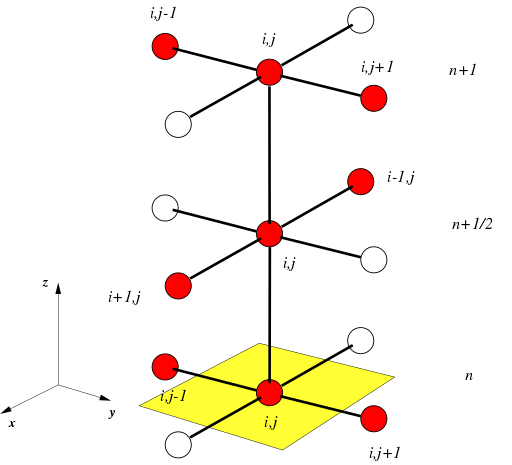
\includegraphics[scale=0.5]{ADI-stencil.png}
\label{fig: ADI_stencil}
\caption{Courtesy: wikipedia.
This stencil portraits the working of the ADI scheme, the first half time step from $t=n$ to $t = n +\frac{1}{2}$ depends implicitly on the cells with coordinates $(i+1,j)$, $(i,j)$ and $(i-1,j)$. The second half time step to $t = n+1$ depends implicitly on cells $(i,j+1)$, $(i,j)$ and $(i,j-1)$.}
\end{figure}

In a more simple form, this can be written as:
\begin{align}
\left(1 + \frac{\Delta t D1_{i+1,j}^{n}}{\Delta x^2} + \frac{\Delta t D1_{i,j}^{n}}{\Delta x^2} \right) E_{i,j}^{n+\frac{1}{2}} - \frac{\Delta t D1_{i+1,j}^{n}}{\Delta x^2} E_{i+1,j}^{n+\frac{1}{2}} - \frac{\Delta t D1_{i,j}^{n}}{\Delta x^2} E_{i-1,j}^{n+\frac{1}{2}} = b_{i,j}
\end{align}
where $b_{i,j} = \left(1 + \frac{\Delta t D2_{i,j+1}^{n}}{\Delta y^2} + \frac{\Delta t D2_{i,j}^{n}}{\Delta y^2}\right) E_{i,j}^{n} + \frac{\Delta t D2_{i,j+1}^{n}}{\Delta y^2} E_{i,j+1}^{n} + \frac{\Delta t D2_{i,j}^{n}}{\Delta y^2} E_{i,j-1}^{n}$
Or in matrix form:
\begin{align}
&\begin{bmatrix}
\ddots & \ddots & & &\\
\ddots & \left(1 + \frac{\Delta t D1_{i,j}^{n}}{\Delta x^2} + \frac{\Delta t D1_{i-1,j}^{n}}{\Delta x^2} \right) & -\frac{\Delta t D1_{i,j}^{n}}{\Delta x^2} & & \\
& -\frac{\Delta t D1_{i,j}^{n}}{\Delta x^2} & \left(1 + \frac{\Delta t D1_{i+1,j}^{n}}{\Delta x^2} + \frac{\Delta t D1_{i,j}^{n}}{\Delta x^2} \right) & - \frac{\Delta t D1_{i,j}^{n}}{\Delta x^2} & \\
& & -\frac{\Delta t D1_{i+1,j}^{n}}{\Delta x^2} & \left(1 + \frac{\Delta t D1_{i+2,j}^{n}}{\Delta x^2} + \frac{\Delta t D1_{i+1,j}^{n}}{\Delta x^2} \right) & \ddots \\
& & & \ddots & \ddots
\end{bmatrix} \\
&\times
\begin{bmatrix}
           \vdots                    \\
           E_{i-1,j}^{n+\frac{1}{2}} \\
           E_{i,j}^{n+\frac{1}{2}}   \\
           E_{i+1,j}^{n+\frac{1}{2}} \\
           \vdots
\end{bmatrix} 
=
\begin{bmatrix}
           \cdots & b_{i,j-1} & b_{i,j} & b_{i,j+1} & \cdots
\end{bmatrix}
\end{align}
This is, depending on boundary conditions, a tridiagonal matrix. In \texttt{MPI-AMRVAC}, this matrix system is solved on the entire computational domain and the innermost layer of ghost cells. The boundary conditions on the radiation energy field are applied after the halved time step. This way, the matrix can be kept tridiagonal independent of those boundary conditions. The tridiagonal system is then solved using Thomas' algorithm, which is a simplified form of Gaussian elimination. If the computational grid is $N$ cells by $M$ cells this is an $(N+2) \times (N+2)$ system, and there are $M+2$ such systems to be solved to evolve half a time step. \\

The second half of the time step will be solved implicit in the $y$-direction and explicit in $x$-direction. Notice again the diffusion coefficient can only be updated at the end of the cycle:
\begin{align}
\frac{E_{i,j}^{n+1} - E_{i,j}^{n+\frac{1}{2}}}{\Delta t}
 &= \frac{D1_{i+1,j}^{n}}{\Delta x^2} (E_{i+1,j}^{n+\frac{1}{2}} - E_{i,j}^{n+\frac{1}{2}}) \\
 &- \frac{D1_{i,j}^{n}}{\Delta x^2} (E_{i,j}^{n+\frac{1}{2}} - E_{i-1,j}^{n+\frac{1}{2}}) \\
 &+ \frac{D2_{i,j+1}^{n}}{\Delta y^2} (E_{i,j+j}^{n+1} - E_{i,j}^{n+1}) \\
 &- \frac{D2_{i,j}^{n}}{\Delta y^2} (E_{i,j}^{n+1} - E_{i,j-1}^{n+1})
\end{align}
And this system, of course, has a matrix notation completely analogous to the one in the first half of the time step, which can be solved in an analogous way. This time there are $N+2$ matrices of size $(M+2) \times (M+2)$ to be solved. \\

The accuracy of this scheme can be checked by computing and comparing both the left hand side and right had side of equation \eqref{eq: Error_control} after calculating $E^{n+1}$. The error is defined by taking the maximum value of the difference of the LHS and RHS weighted with the ratio of the radiative energy and the hydrodynamical time step \citep{Turner12001}:
\begin{align}
Error = \max_{i,j} \left(\frac{\frac{E^{n+1} - E^{n}}{\Delta t} -  \vec{\nabla} \cdot \left(D \nabla E\right)}{E^{n}/dt} \right) \label{eq: Error}
\end{align}

In a completely correct computation, the left hand side would correspond exactly to the right hand side, however due to numerical computations and assumptions this will almost never truly hold.\\

 Test calculations show that this error is often rather large, depending on the distribution of the radiation and density field in the simulation space. A solution is given in \citep{Turner12001} by means of pseudo-time stepping. This method will be explained in the next section.
 
 
\subsection{pseudo-timestepping}
Instead of solving equation \eqref{eq: diffusion} a new variable is introduced, the \emph{pseudotimestep} $w$. The ADI-method is used to solve 
\begin{align}
\partial_w E = \partial_t E  - \vec{\nabla} \cdot \left(D \nabla E\right)
\end{align}
which reduces to \eqref{eq: diffusion} when $\partial_w E = 0$. The pseudo-time step $\Delta w$ can be adjusted independently from the hydrodynamical time step and is increasing in size to converge toward a $w$-stationary state where $\partial_w E = 0$ \citep{Turner12001}.\\

The implicit scheme to evolve half a pseudo-time step from $m$ to $m + \frac{1}{2}$, implicit in the $x$-direction, looks like:
\begin{align}
\frac{E_{i,j}^{m+\frac{1}{2}} - E_{i,j}^{m}}{\Delta w} 
 &= \frac{E_{i,j}^{m+\frac{1}{2}} - E_{i,j}^{n}}{\Delta t} \\
 &- \frac{D1_{i+1,j}^{n}}{\Delta x^2} (E_{i+1,j}^{m+\frac{1}{2}} - E_{i,j}^{m+\frac{1}{2}}) \\
 &+ \frac{D1_{i,j}^{n}}{\Delta x^2} (E_{i,j}^{m+\frac{1}{2}} - E_{i-1,j}^{m+\frac{1}{2}}) \\
 &- \frac{D2_{i,j+1}^{n}}{\Delta y^2} (E_{i,j+j}^{m} - E_{i,j}^{m}) \\
 &+ \frac{D2_{i,j}^{n}}{\Delta y^2} (E_{i,j}^{m} - E_{i,j-1}^{m})
\end{align}

Where, again, the Diffusion coefficient is considered constant throughout the full hydrodynamical time step. This corresponds to a similar tridiagonal matrix equation which has to be solved for every pseudo-time step. Following, the size of the pseudo-time step $\Delta w$ is exponentially increasing in size per iteration $m = 1 ... W$ and is given by:
\begin{align}
\Delta w = \Delta w_0 \left(\frac{\Delta w_1}{\Delta w_0} \right)^\frac{m-1}{W-1}
\end{align}

$\Delta w_0$ And $\Delta w_1$ are one quarter of the size of a grid cell and one quarter of the size of the numerical domain, respectively. The error of this combined ADI-pseudo-time step method is measured after $W$ pseudo-time steps using \eqref{eq: Error}, if it is too large $W$ and $\Delta w_1$ are increased whilst $\Delta w_0$ is decreased. If this still doesn't suffice, the above scheme can be applied twice to half a hydrodynamical time step, four times to a quarter hydrodynamical time step, etc. In the testcases described in section \ref{section: res: diff_test}, typically ...4... pseudo-time teps where necessary to reach convergence, depending on the hydro time step.

\subsection{Bisection Implicit scheme} \label{subsection: BIS}
Solving for the source terms in the gas and radiation energy equations happens with another implicit scheme. 
\begin{align}
e^{n+1} - e^n &= \Delta t \left( -4\kappa \sigma \left(\frac{(\gamma - 1)e^{n+1}}{\rho}\right)^4 + c \kappa E^{n+1} \right) \\ 
E^{n+1} - E^n &= \Delta t \left( +4\kappa \sigma \left(\frac{(\gamma - 1)e^{n+1}}{\rho}\right)^4 - c \kappa E^{n+1} -\nabla \vec{v} P^{n+1} \right)
\end{align} 
This can be rewritten as:
\begin{align}
e^{n+1} - e^n &= -a_1 \left( e^{n+1}\right)^4 + a_2 E^{n+1}  \\ 
E^{n+1} - E^n &= a_1 \left( e^{n+1} \right)^4 - a_2 E^{n+1} - a_3 E^{n+1} 
\end{align}
where $a_1 = 4\kappa \sigma \left(\frac{(\gamma - 1)}{\rho^{n+1}}\right)^4 \Delta t$, $a_2 = c \kappa \Delta t$ and $a_3 = \frac{\nabla \vec{v} P^{n+1} }{E^{n+1}} \Delta t$. Manipulation of the equations returns:
\begin{align}
E^{n+1} &= \frac{a_1 \left( e^{n+1} \right)^4 + E^n}{1 + a_2 + a_3} \label{eq: E_src}
\end{align}
And
\begin{align}
\left( e^{n+1} \right)^4 &+ \frac{1 + a_2 + a_3}{a_1 + a_3}e^{n+1} -  \frac{(1 + a_2 + a_3)e^n + a_2 E^n}{a_1 + a_3} = 0 \label{eq: Poly}
\end{align}

Equation \eqref{eq: Poly} is a $4^{th}$ degree polynomial in $e^{n+1}$, with a single root between $0$ and $\frac{1 + a_2 + a_3}{a_1 + a_3}$. This is solved for $e^{n+1}$ using the bisection method to calculate the contribution of the radiative heating and cooling to the gas energy. The newly calculated $e^{n+1}$ is then plugged in equation \eqref{eq: E_src} to find the contribution of the radiative heating and cooling, and the photon tiring to the radiation energy.

\section{Dimensionless problem}
Computationally, floating point values are the most precise around unity. For this reason, it is preferable to rescale physical quantities such as $\rho$, $\vec{v}$, $e$, ... with values typical to the simulation domain. \texttt{mpi-AMRVAC} already does port of this for us, in the user module, one can define either the units for either number density, temperature  and length ($N_0$, $T_0$, $l_0$) or  number density, velocity  and length ($N_0$, $v_0$, $l_0$). The other units will be then computed from these quantities using the following relations:
\begin{align}
\rho_0 &= \mu m_p N_0 \\
   p_0 &= \gamma N_0 k_b T_0 \\
   v_0 &= \sqrt{\frac{p_0}{\rho_0}} \\
   t_0 &= \frac{l_0}{v_0}
\end{align}
Calculations in amrvac are always done with unit less quantities, in HD these are: $\tilde{\rho} = \frac{\rho}{\rho_0}$, $\tilde{\vec{v}} = \frac{\vec{v}}{\vec{v}_0}$, $\tilde{p} = \frac{p}{p_0}$ and $\tilde{e} = \frac{e}{p_0}$. Using this, we can transform the continuity equation \eqref{eq: hd_rho} to dimensionless units:
\begin{align}
\frac{t_0}{\rho_0} \frac{\partial}{\partial t} \rho  + \frac{t_0}{\rho_0} \vec{\nabla} \cdot \left( \rho \vec{v}  \right) &= \frac{t_0}{\rho_0} S_\rho \\
\frac{\partial}{\partial \tilde{t}} \tilde{\rho} + \tilde{\nabla} \left( \tilde{\vec{v}} \tilde{\rho} \right) &= \tilde{S}_\rho
\end{align}
Where $\nabla$ has the units of reciprocal length and $\tilde{S}_\rho \def \frac{t_0}{\rho_0} S_\rho$. Equivalently, for the momentum equation \eqref{eq: hd_mom} and the gas energy equation \eqref{eq: hd_e}:
\begin{align}
\frac{\partial}{\partial \tilde{t}} \left(\tilde{\rho} \tilde{\vec{v}} \right) + \tilde{\vec{\nabla}} \left(\tilde{\vec{v}} \tilde{\rho}  \tilde{\vec{v}} + \tilde{p} \right) &= \tilde{S}_{\rho \vec{v}} \\
\frac{\partial}{\partial \tilde{t}} \tilde{e} + \tilde{\vec{\nabla}} \left(\tilde{\vec{v}} \tilde{e} + \tilde{\vec{v}} \tilde{p} \right) &= \tilde{S}_e \\
\end{align}
$\tilde{S}_{\rho \vec{v}} = S_{\rho \vec{v}} \frac{t_0}{\rho_0 v_0}$ and $\tilde{S}_e = S_e \frac{t_0}{e_0}$ are the momentum and energy equation source terms. For the RHD equations this will rescale the physical constants:
\begin{align}
	\tilde{S}_{\rho \vec{v}} &=  \frac{\kappa \rho}{c} \vec{F} \frac{t_0}{\rho_0 v_0} \\
							 &=  \frac{\tilde{\kappa}\tilde{\rho}}{\tilde{c}} \tilde{\vec{F}} \\
	\tilde{S}_e &= -4\pi \kappa\rho B \frac{t_0}{e_0}  + c \kappa \rho E \frac{t_0}{e_0} \\
				&= -4 \tilde{\sigma} \tilde{\kappa} \tilde{T}^4 + \tilde{c} \tilde{\rho} \tilde{E}
\end{align}
The rescaled Stefan-Boltzmann constant $\tilde{\sigma}$, the rescaled speed of light $\tilde{c}$ and the rescaled opacity $\tilde{\kappa}$ are given by $\tilde{\sigma} = \frac{\sigma T_0^4}{e_0 v_0}$, $\tilde{c} = \frac{c}{v_0}$ and $\tilde{\kappa} = \kappa v_0 t_0$. The unit of the radiation energy density and radiation flux can also be defined: $E_0 = e_0$ and $F_0 = \rho_0 v_0^3$. These are used to transform the RHD equation for radiation energy \eqref{eq: rhd_e_r} and the FLD closure relation \eqref{eq: fld_closing}. 

\section{visualisation}
\texttt{mpi-AMRVAC} output is given in binary .vtu files. Special software such as visit \citep{} and paraview are used to open and analyse the simulation results. The standard output consists of the primitive variables at every simulation cell for a specified number of time steps. Extra output variables can be defined in the user module.


\newpage
\chapter{Results}
The first result is of course a working CAK subroutine and FLD module in mpi-AMRVAC. This is something that didn't exist before and it will open the way toward simulations of new physical regimes where radiation plays a role in the dynamics of the system. In addition to   designing, writing and benchmarking the software, there are also a few first scientific results. These will be described in this chapter.

\section{CAK-Theory}
\subsection{Massive star stellar wind}
The CAK momentum equation for a point like star, so when disregarding the finite disk correction factor, has an analytic solution. This solution will be derived below, based on \citep{Owocki2003}, for comparison with the numerical models. Afterwards, the corrections for finite disks will be mentioned. Begin by writing down the steady state momentum equation in 1D spherical coordinates, disregarding the pressure term. The pressure gradient will be orders of magnitude smaller than the gravitational and radiative accelerations due to the low density environment. 
\begin{align}
\nabla_r \left(v_r \rho v_r \right) = \rho g_{CAK} + \rho g_{e} - \rho g_{grav}
\end{align}
Using the steady state continuity equation and the electron scattering Eddington factor $\Gamma_e$ this can be written as:
\begin{align}
v \frac{d v}{d r} = g_{CAK} + (\Gamma_e-1) \frac{G M_*}{r^2} \label{eq: CAK_mom}
\end{align}
Lets introduce two new variables: $x = 1- \frac{R_*}{r}$ is a dimensionless inverse radius coordinate, and $w = \frac{v^2}{v_{esc}^2}$ is the kinetic energy as ratio of the kinetic energy at effective escape velocity. The effective escape velocity is similar to the general expression for escape velocity, but corrected for electron scattering force: $v_{esc} = \sqrt{(1- \Gamma_e) \frac{2 G M_* }{R_*}}$. Using the notation $w' = \frac{dw}{dx} = \frac{dw}{dr}\frac{dr}{dx}$ and $v' = \frac{dv}{dx} = \frac{dv}{dr} \frac{dr}{dx}$, $w'$ can be written as:
\begin{align}
w' = vv' \frac{r^2}{G M_* (1- \Gamma_e)}
\end{align}
Fill in $v\frac{dv}{dr}$ from equation \eqref{eq: CAK_mom}, where $vv' = v \frac{dv}{dr} \frac{dr}{dx} = v \frac{dv}{dr} \frac{r^2}{R_*^2}$:
\begin{align}
w' &= v \frac{dv}{dr}  \frac{r^2}{R_*^2} \frac{r^2}{G M_* (1- \Gamma_e)} \\
   &= \left( g_{CAK} + (\Gamma_e-1) \frac{G M_*}{r^2} \right)  \frac{r^2}{R_*^2} \frac{r^2}{G M_* (1- \Gamma_e)}\\
   &= C w'^\alpha - 1 \label{eq: CAK_w}
\end{align}

SOMETHING FISHY WITH $\frac{r^2}{R_*^2}$ HERE\\

Where, if we define the constant mass loss rate $\dot{M} = 4\pi r^2 \rho(r) v(r) = c^{ste}$, C is given by:
\begin{align}
C = \frac{1}{1-\alpha} \left(\frac{\bar{Q}\Gamma_e}{1-\Gamma_e} \right)^{1-\alpha} \left(\frac{L_*}{\dot{M}c^2}\right)^\alpha \label{eq: CAK_Cste}
\end{align}
$C$ Depends inversely on the mass loss rate $\dot{M}$, depending on the value of $C$, equation \ref{eq: CAK_w} has either zero ($C < C_{crit}$), one ($C = C_{crit}$) or two ($C = C_{crit}$) solutions. A low value for $C$ leads to a high $\dot{M}$, so the solution with the maximal mass loss rate is the single solution at $C = C_{crit}$ The critical value for $C$ occurs when the function $C w'^\alpha$ intersects function $1 + w'$ in a tangent point. This occurs at critical argument $w'_{crit} = \frac{\alpha}{1-\alpha}$ for critical $C$-value $C = \frac{\alpha^{-\alpha}}{(1-\alpha)^{1-\alpha}}$. One can now integrate over $w'_{crit}$ to obtain a velocity profile.
\begin{align}
w'_{crit} &= \frac{\alpha}{1-\alpha} \\
v(r) &= v_{esc} \sqrt{\frac{\alpha}{1-\alpha}} \left(1 - \frac{R_*}{r} \right)^\frac{1}{2}
\end{align}
Where, when $r\rightarrow\infty$, $v(\infty) \rightarrow v_{esc} \sqrt{\frac{\alpha}{1-\alpha}} = v_\infty$. This type of velocity field follows a beta velocity law ($v = v_\infty (1-R/r)^\beta$), where in this case $\beta = 0.5$. The maximal CAK mass loss rate connected to the critical value $C_{crit}$ can also be analytically determined by solving equation \ref{eq: CAK_Cste} for $\dot{M}$:
\begin{align}
\dot{M}_{CAK} = \frac{L_*}{c^2} \frac{\alpha}{1-\alpha}\left(\frac{\bar{Q}\Gamma_e}{1-\Gamma_e}\right)^{\frac{1-\alpha}{\alpha}}
\end{align}

Let's now have a look at some corrections that can be made when considering a finite disk instead of a point source. Define the rescaled correction factor as $f_* = \frac{f_{fd}}{f}$ and the rescaled constant $C_* = C f$, where $f$ is the finite disk correction factor at the stellar surface. At the stellar surface, $r \rightarrow R_*$, $v \rightarrow 0$ and $dv/dr \sim v/r$, plug this in in equation \ref{eq: fin_disk_corr} gives $f_{fd}(R_*) = f \sim \frac{1}{1+\alpha}$. Equation \ref{eq: CAK_w} now rescales to:
\begin{align}
w' = f_* C_* (w')^\alpha - 1 
\end{align}
Analogous reasoning as before leads to an adjusted CAK mass loss rate $\dot{M}_{fd}$. This mass loss rate will be lower than the point source mass loss rate, because $f \sim \frac{1}{1+\alpha}  < 1$.
\begin{align}
\dot{M}_{fd} = \frac{\dot{M}_{fd}}{(1+\alpha)^\frac{1}{\alpha}}
\end{align} 

ADJUST PLOTS 'N' STUFF


Now that we have testable observables (the steady state CAK mass loss rate $\dot{M}_{CAK}$ and the steady state velocity and density profiles $v(r), \rho(r)$), it is time time to run some simulations and compare the outcomes to the analytical solutions.\\

The CAK source term is used to model the wind of a massive O-type star. A star of luminosity $L = 8\cdot 10^5 L_\odot$ and mass $M = 50 M_\odot$ is taken at as the mass driver (see table \ref{tab: CAK_res}). \\

\begin{table}[]
\centering
\caption{Top part: Parameters used in setting the initial conditions of the wind based on \citep{Sundqvist2013}. Bottom part: Fitted parameters.}
\label{tab: CAK_res}
\begin{tabular}{llll}
\hline
\hline
\multicolumn{4}{l}{Stellar wind parameters}                                           \\
\hline
$R/R_\odot$              &             & $20$ &\\
$L/L_\odot$              &             &  $8\cdot10^{5}$  &\\
$M/M_\odot$              &             & $50$ &\\
$T[K]$                   &             & $4\cdot10^{4}$ &\\
$c_{adiab}[\frac{m}{s}]$ &             & $2.3\cdot 10^{6}$ &\\
$\bar{Q}$ 				 &             & $2000$ &\\
$\alpha$                 &             & $0.67$ &\\
$\rho_0[\frac{g}{cm^3}]$ &             & $2.2\cdot 10^{-12}$ &\\
\hline
\hline
\multicolumn{4}{l}{Fitting parameters}                                                \\
                         & theoretical & best fit point source & best fit finite disk \\
\hline
$\beta$                  & $0.5$       & $0.543\pm 0.001$      &  $0.761 \pm 0.001$   \\
$v_{\infty}/c_{adiab}$   & $45.69$     & $33.14\pm 0.04$       &  $149.4 \pm 0.1$     \\
$\dot{M}[\frac{M_\odot}{yr}]$ & $4.1 \cdot 10^{-6}$  & $(3.4 \pm 0.4)10^{-7}$&  $(1.8\pm0.2)10^{-7}$ \\           
\end{tabular}
\end{table}




The tricky bit in the setup of this simulation is choosing correct lower boundary conditions. The stellar wind is launched from the stellar surface and begins with a subsonic velocity. Computationally this is controlled by setting the lower boundary density $\rho_0$. If the density on the lower bound is too high, the simulation domain begins "too deep" in the stellar atmosphere, the equations become too stiff \citep{Sundqvist2013}. If $\rho_0$ is too low, the simulation domain begins in the supersonic region.\\

As initial condition, the velocity field is taken as a beta velocity law with $\beta > 0.5$, this leads to higher velocity and thus a supercritical solution. The initial density can be derived from the mass los rate: $\rho = \frac{\dot{M}_{CAK}}{4\pi r^2 v}$. The velocity profile should relax towards the critical solution where $\beta = 0.5$ for the point source driven and $\beta = 0.8-1$ \citep{Owocki2003} for the finite disk driven wind.\\

The lower boundary for the radial velocity is set according to the continuity equation $\nabla (\rho v) = 0$, meaning $v_0 = \frac{\rho_1 v_1}{\rho_0}$. Initial conditions are evolved towards an almost stable, nearly steady state, results of the simulations and their analytical counterparts are plotted in figures \ref{fig: CAK_PS_v} and \ref{fig: CAK_PS_rho}.\\

A beta-velocity law is fitted trough the numerical velocity profile to get the wind characteristics. The actual mass loss rate can be calculated by fitting $\rho_{fit} = \frac{\dot{M}}{4\pi r^2 v_{fit}}$ to the density profile with $\dot{M}$ as a free parameter. Results are tabulated in table \ref{tab: CAK_res}

\begin{figure}
\centering
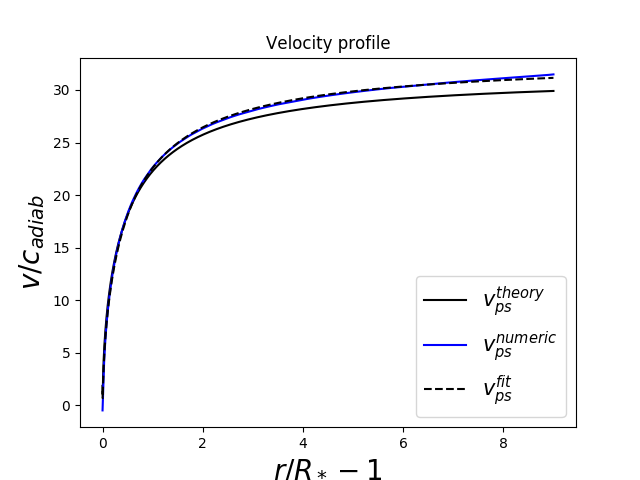
\includegraphics[width = \textwidth]{CAK_velocity_profile.png}
\caption{The velocity profile for the source point like star CAK wind. In dashed lines the initial conditions, in green the analytical steady state solution and in blue and red the solutions after 0.5 and 50 times $t = R_*/c_{adiab}$.}
\label{fig: CAK_PS_v}
\end{figure}

\begin{figure}
\centering
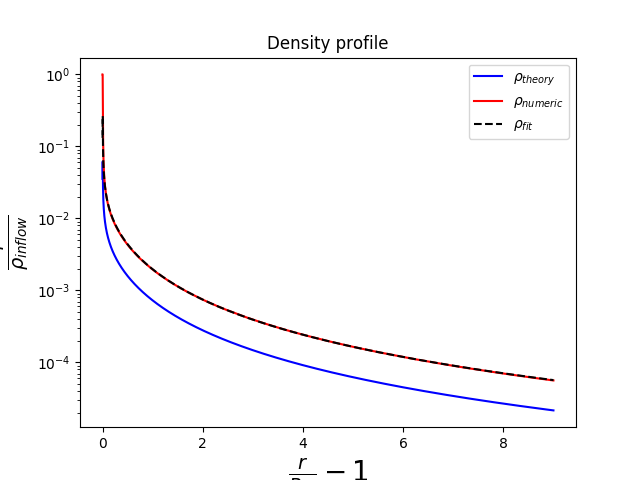
\includegraphics[width = \textwidth]{CAK_density_profile.png}
\caption{The density profile for the source point like star CAK wind. In dashed lines the initial conditions, in green the analytical steady state solution and in blue and red the solutions after 0.5 and 50 times $t = R_*/c_{adiab}$.}
\label{fig: CAK_PS_rho}
\end{figure}


%\begin{figure}
%\centering
%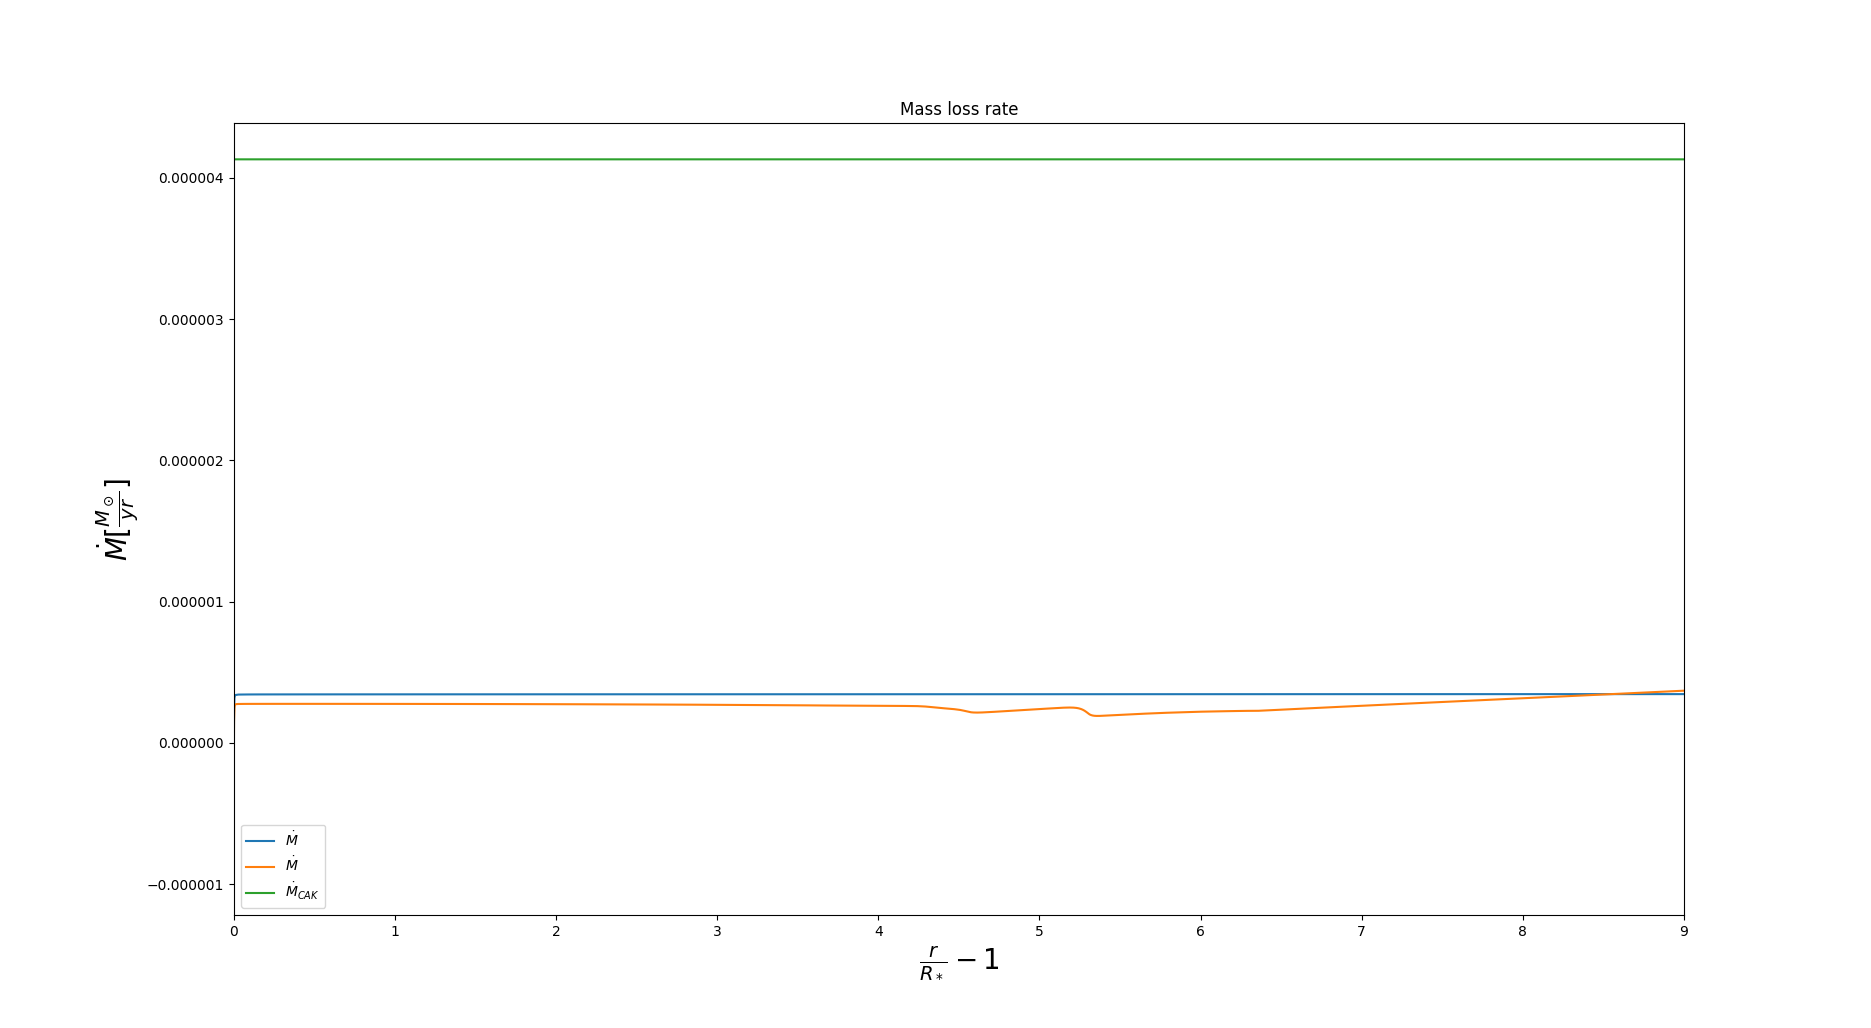
\includegraphics[width = \textwidth]{CAK_mass_loss.png}
%\caption{The mass loss rate profile for the source point like star CAK wind. In dashed lines the initial conditions, in green the analytical steady state solution and in blue and red the solutions after 0.5 and 50 times $t = R_*/c_{adiab}$.}\label{fig: CAK_PS_M_dot}
%\end{figure}

When accounting for the finite disk correction, the steady state velocity profile doesn't follow a $\beta = 0.5$ velocity law, results are shown in figures \ref{fig: CAK_PS_v} and \ref{fig: CAK_PS_rho}, the correction factor is plotted in figure \ref{fig: fd_factor}. 

\begin{figure}
\centering
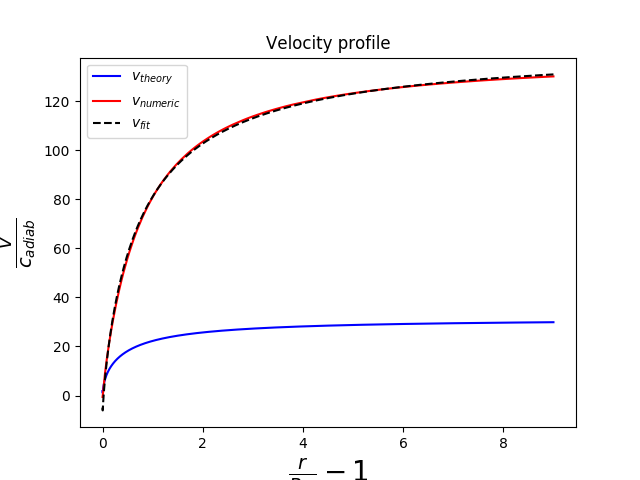
\includegraphics[width = \textwidth]{CAK_fd_velocity_profile.png}
\caption{The velocity profile for the finite disk corrected CAK wind. In dashed lines the initial conditions, in green the analytical steady state solution and in blue and red the solutions after 0.5 and 50 times $t = R_*/c_{adiab}$.}
\label{fig: CAK_fd_v}
\end{figure}

\begin{figure}
\centering
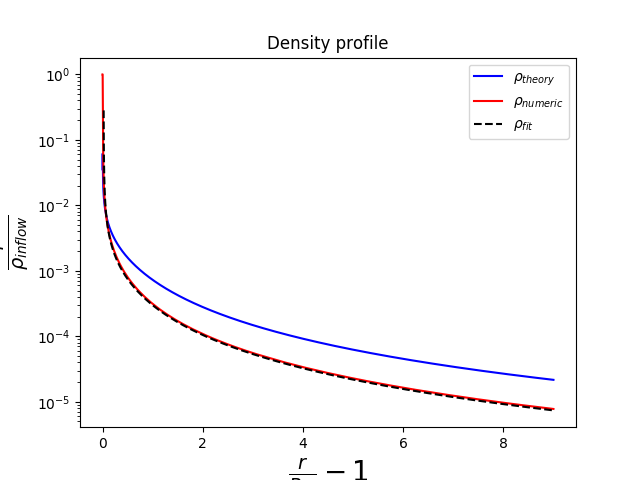
\includegraphics[width = \textwidth]{CAK_fd_density_profile.png}
\caption{The density profile for the finite disk corrected CAK wind. In dashed lines the initial conditions, in green the analytical steady state solution and in blue and red the solutions after 0.5 and 50 times $t = R_*/c_{adiab}$.}
\label{fig: CAK_fd_rho}
\end{figure}
%
%
%\begin{figure}
%\centering
%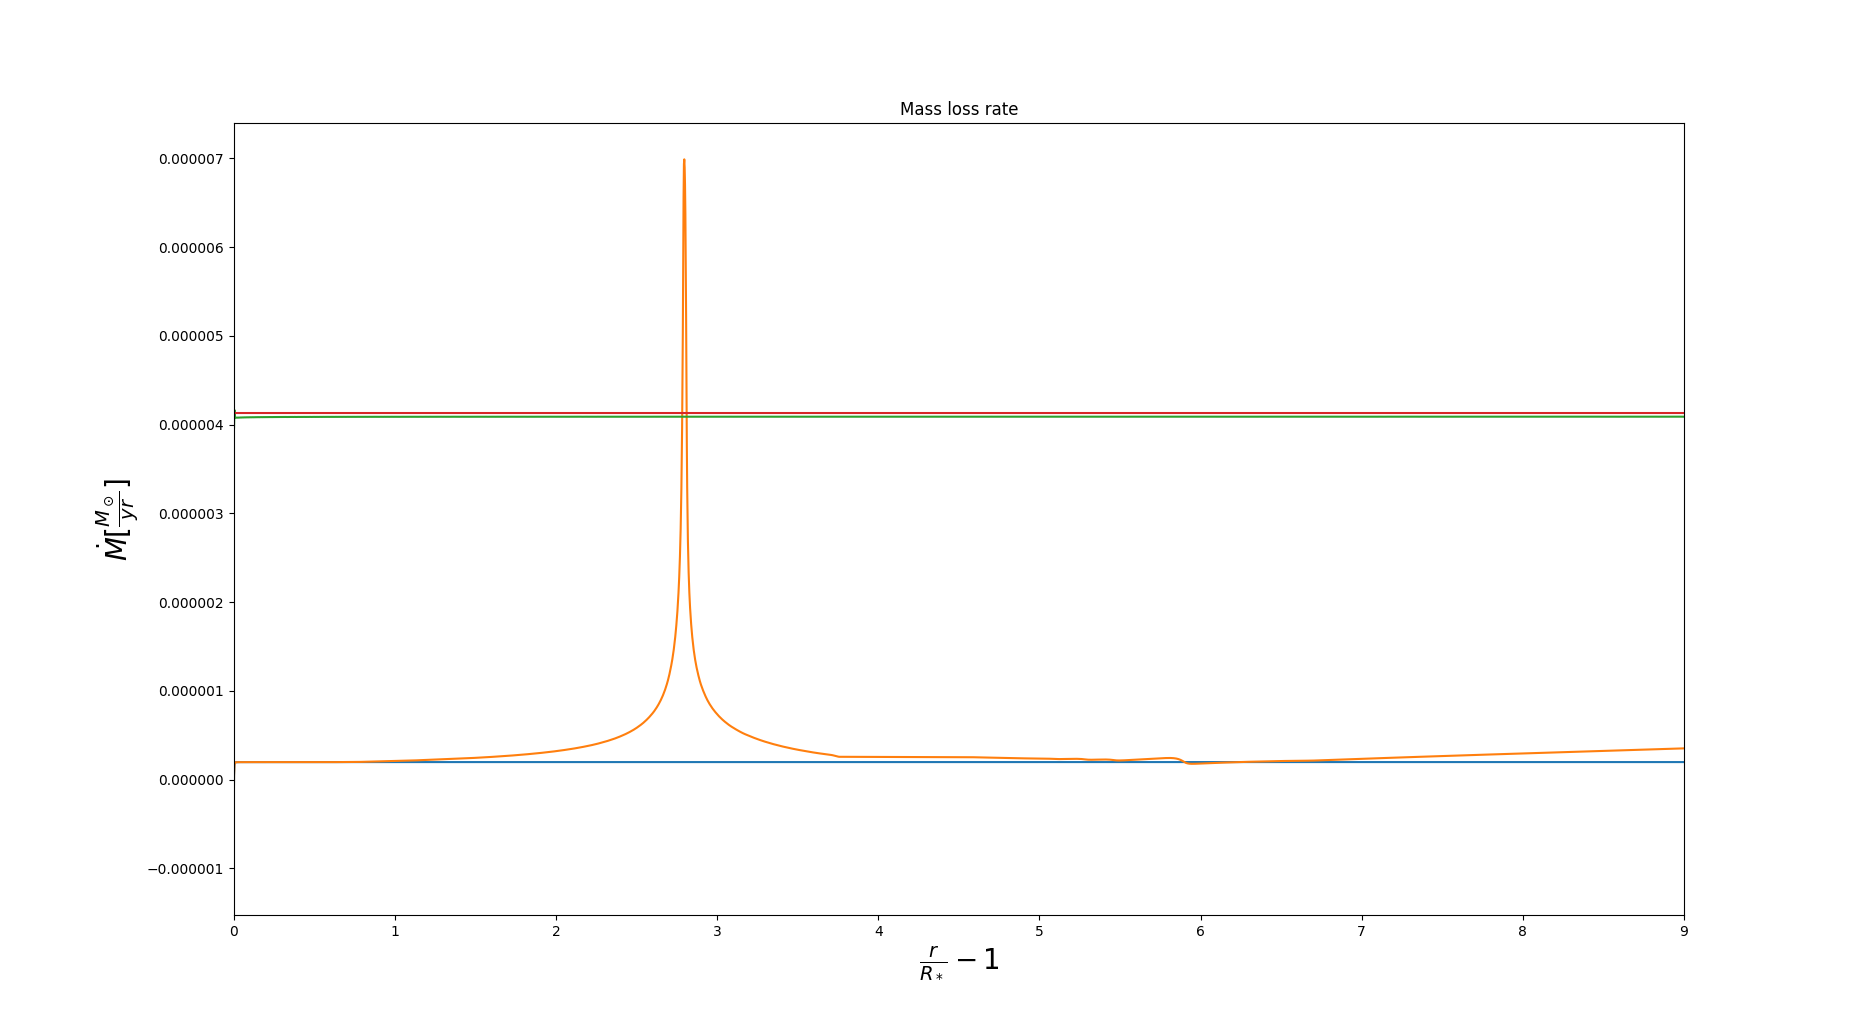
\includegraphics[width = \textwidth]{CAK_fd_mass_loss.png}
%\caption{The mass loss rate profile for the finite disk corrected CAK wind. In dashed lines the initial conditions, in green the analytical steady state solution and in blue and red the solutions after 0.5 and 50 times $t = R_*/c_{adiab}$.}
%\label{fig: CAK_fd_M_dot}
%\end{figure}

\begin{figure}
\centering
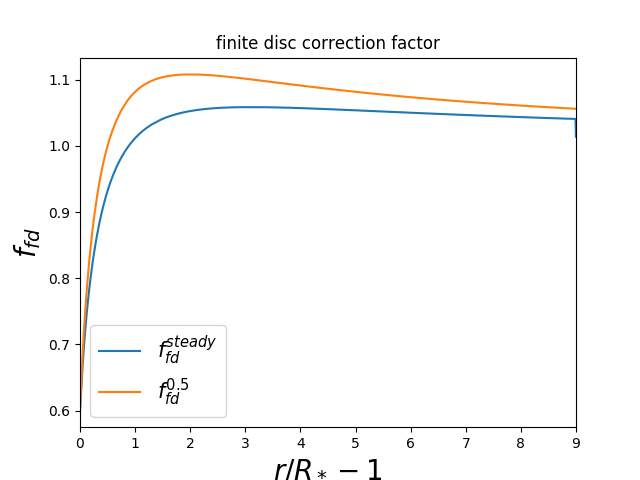
\includegraphics[width = \textwidth]{CAK_fd_factor.png}
\caption{•}
\label{fig: fd_factor}
\end{figure}

%Closing
Having now succesfully implemented and benchmarked a radiative line driving module into \texttt{MPI-AMRVAC}, future work will be done in for exemple extension toward 2D and 3D simulations,  interaction of stellar winds with orbiting compact objects such as BH's, NS's or WD's (X-ray binaries) \citep{Mellah2017}.


\section{Flux Limited Diffusion}
The diffusion model is first tested against some analytical results, these tests will give us knowledge on how accurately we can interpret the simulations of physical phenomena. The diffusion term and advection term are both tested separately by comparison to an exact solution and the photon tiring, radiative cooling and radiative heating source terms are tested together versus a Runge-Kutta solver of a simplified problem.

\subsection{Testcase 1: Advection and Diffusion}\label{section: res: diff_test}
The advection problem and the diffusion problem, solved by the already existing Riemann solver and the new ADI solver respectively can be tested by comparing them to simplified situation where an exact analytical solution can be found. The Riemann solver is nothing new, it's just a matter of checking the correct implementation in \texttt{MPI-AMRVAC}. The problem is tested on a numerical domain with constant density, a constant velocity, a constant gas energy density and an initial radiation energy density $E_0(x,y,t)$ given by:
\begin{align}
E_0(x,y,t) = 2 + \sin(2 \pi x) \sin(2 \pi y)
\end{align}
If diffusion and other source terms are ignored, the radiation field will evolve as
\begin{align}
E^{adv}(x,y,t) = 2 + \sin(2 \pi (x-v_x t)) \sin(2 \pi (y-v_y t))
\end{align}
If diffusion is switched on but the advection is ignored by fixing the velocity field to $\vec{0}$ every iteration, and the diffusion coefficient is chosen constant at $D = 1$, the field evolves as
\begin{align}
E^{diff}(x,y,t) = 2 + \exp(-8 \pi^2 t) \sin(2 \pi x) \sin(2 \pi y)
\end{align}

Function $E_0(x,y,t)$ describes a series of dots of more and less radiative energy, see figure \ref{fig: InitCond_test}. The numerical domain is chosen in such a way that there is one region of lower and one region of higher energy in each direction, $-0.5 \leq x \leq 0.5$, $0 \leq y \leq 1$. In time, the diffusion test runs until the amplitude of the dots diminish by two orders of magnitude $\exp(-8 \pi^2 t)  = 10^{-1}$ and the advection test tuns until a point has passed the computational domain twice $ \min(v_x, v_y) t = 2 $. Boundary conditions are set periodical. Computational result $\tilde{E}$ can be compared with the analytical results to define the residuals:
\begin{align}
RES^{adv} &= \left|\frac{\tilde{E}^{adv} - E^{adv}}{E^{adv}}\right| \\
RES^{diff} &= \left|\frac{\tilde{E}^{diff} - E^{diff}}{E^{diff}}\right| 
\end{align}

Which are plotted for different timesteps in figure \ref{fig: test_advection} and \ref{fig: test_diffusion} together with the numerical solutions $\tilde{E}^{adv}$ and $\tilde{E}^{diff}$


\begin{figure}
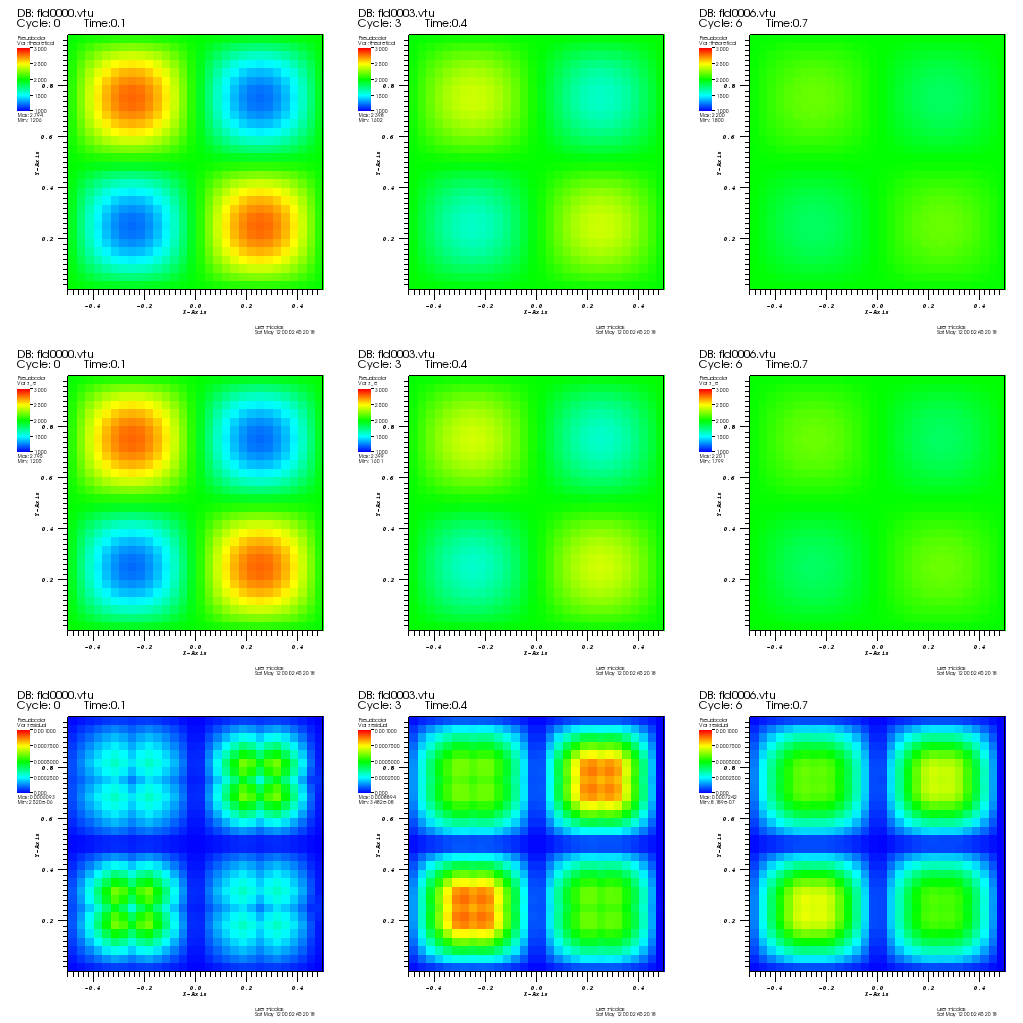
\includegraphics[width = \textwidth]{visit0001.png}
\label{fig: test_diffusion}
\caption{top: theoretical solution $E^{diff}$, middle: computed result $\tilde{E}^{diff}$ and bottom: residual $RES^{diff}$. Left: $0.1 t_0$, middle $0.4 t_0$ and right $0.7 t_0$. The scale goes from $1$ to $2$ for the upper two rows and form 0 to 0.01 for the bottom row.}
\end{figure}

\begin{figure}
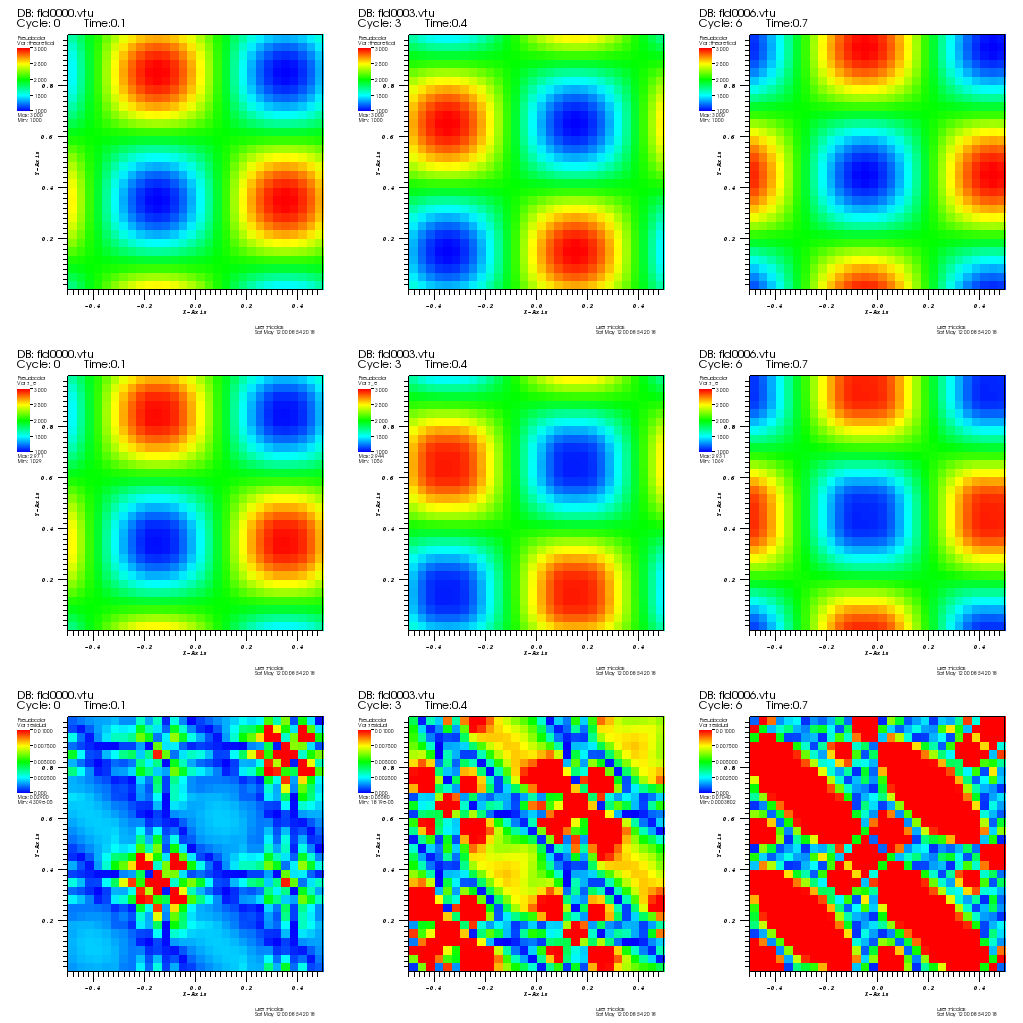
\includegraphics[width = \textwidth]{visit0002.png}
\label{fig: test_advection}
\caption{top: theoretical solution $E^{adv}$, middle: computed result $\tilde{E}^{adv}$ and bottom: residual $RES^{adv}$. Left: $0.1 t_0$, middle $0.4 t_0$ and right $0.7 t_0$. The scale goes from $1$ to $2$ for the upper two rows and form 0 to 0.001 for the bottom row.}
\end{figure}



\subsection{Testcase 2: Photon Tiring, Heating and Cooling}
To test the implicit bisection scheme used for adding the photon tiring, radiative heating and radiative cooling source terms, we make comparisons with an explicit Runge-Kutta solver. Of course this Runge-Kutta solver is not to be used in the actual code, because the time step chosen in the Runge-Kutta solver will be orders of magnitude smaller. The equation at hand is:
\begin{align}
\frac{d e}{dt} = c \rho \kappa E - 4 \rho \kappa \sigma T^4
\end{align}
Equivalently the test can be ran on the source terms for the radiative energy equation $\frac{dE}{dt} = - \vec{\nabla} \cdot \vec{v} P + 4\pi \kappa\rho B - c \kappa \rho E$ , where the photon tiring term would drop out due to the velocity field being zero.
Except for the gas energy density, all primitive variables ($\rho = \rho_0$, $\vec{v} = 0$ and $E = E_0$) are kept constant. The computational domain is taken as small as possible and radiative diffusion is switched off. \\

The system would be in radiative equilibrium when $c \rho \kappa E = 4 \rho \kappa \sigma T^4$. Using $T =  \frac{p}{\rho} \frac{m_p \mu}{k_b}= \frac{(\gamma - 1)e}{\rho} \frac{m_p \mu}{k_b}$, on can compute the equilibrium gas energy.
\begin{align}
e_{eq.} = \frac{\rho}{\gamma - 1} \frac{k_b}{m_p \mu}\left( \frac{c E}{4 \sigma} \right)^\frac{1}{4}
\end{align}
Different initial conditions are chosen for $e_0$ ranging from $10^2 e_{eq.}$ to $10^{-10} e_{eq.}$. Comparisons between the bisection method and a simple Runge-Kutta solver are plotted in figure \ref{fig: test_sourceterms}. Remember that the implicit bisection method uses a time step which is several orders of magnitude larger than the explicit Runge-Kutta method.

\begin{figure}
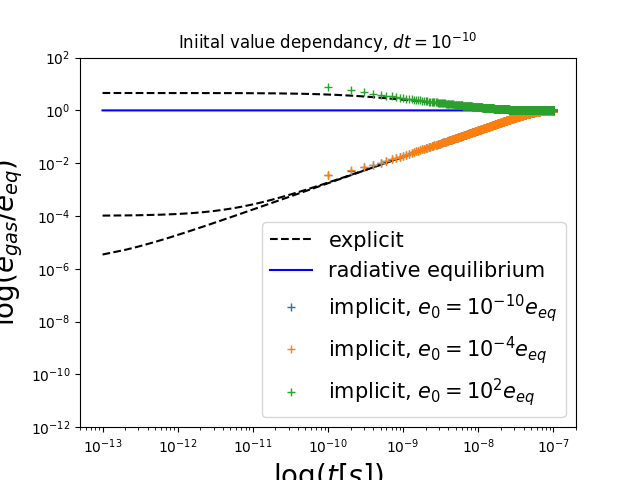
\includegraphics[width = \textwidth]{test_sourceterms.png}
\label{fig: test_sourceterms}
\caption{Comparison between the implicit method (red) and explicit method (black) for computing the radiation heating and cooling sourceterms. The gas energy evolves toward radiative equilibrium (blue) from different initial values. The time step for the implicit method is 3 orders of magnitude larger than the time step for the explicit method.}
\end{figure}

\begin{figure}
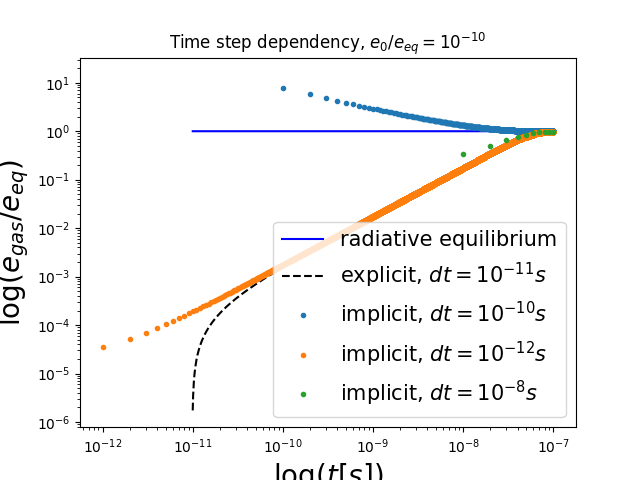
\includegraphics[width = \textwidth]{test_sourceterms_dt.png}
\label{fig: test_sourceterms}
\caption{Comparison between the implicit method (orange, blue, green) and explicit method (black) for computing the radiation heating and cooling sourceterms. The gas energy evolves toward radiative equilibrium (blue) with different time steps for the implicit method.}
\end{figure}

\subsection{Isothermal Thomson Atmosphere} \label{section: IsoAtm}
A first practical use for the FLD module is modelling a stellar atmosphere surrounding a massive star. For convenience, the atmosphere will be considered isothermal and plane parallel, so the flux in the initial condition and the gravitational acceleration are constant. Let's also assume the only absorption an emission is done by means of electron scattering (Thomson atmosphere), with a constant opacity $\kappa$. The model is done in 2D.\\

The initial conditions are crucial in stabilizing simulations. In an isothermal atmosphere, the density and gas pressure decay exponentially on the length of a scale height $H_{eff} = \frac{c_{sound}^2}{g_{eff}}$. Where $g_{eff} = g_{grav}(\Gamma - 1)$ is the sum of radiation and gravitational accelerations. 
\begin{align}
\rho(y) &= \rho_0 \exp \left( -\frac{y}{H_{eff}} \right) \\
 p(y)   &= p_0    \exp \left( -\frac{y}{H_{eff}} \right)
\end{align}

The velocity field is $\vec{0}$ everywhere. Boundary conditions $\rho_0$ and $p_0$ can be computed by defining the optical depth $\tau$. 
\begin{align}
\tau(y) = \int_\infty^{y} \kappa \rho dy  \label{eq: opt_depth}
\end{align}
Let $dm = \rho dy$, if this is substituted in \eqref{eq: opt_depth} we get an expression for the column mass in terms of opacity and optical depth:
\begin{align}
\frac{\tau}{\kappa} = \int_0^{m'} \rho dm
\end{align}


In a static medium, the gravitational and radiative acceleration of the gas is countered by the gas pressure gradient. Concerning the radiation field, one can make a similar statement . The radiative acceleration is countered by the radiation pressure gradient:
\begin{align}
\frac{dp}{dy} \frac{1}{\rho} &= \frac{dp}{dm} = -g_{grav}(1 - \Gamma) \label{eq: p_cond} \\
\frac{dP}{dy} \frac{1}{\rho} &= \frac{dP}{dm} = -g_{grav} \Gamma \label{eq: P_cond}
\end{align}
Manipulating equation \label{eq: p_cond} and substituting the expression for column mass leads to the following relation between optical depth and gas pressure:
\begin{align}
\int_0^{p_0} dp &= -g_{grav}(1 - \Gamma) \int_0^{m_0} dm
\end{align}
This expression can be integrated towards a value for $p_0$ at a given optical depth $\tau_0$. \eqref{eq: P_cond} And \eqref{eq: p_cond} can by divided by one another to get a relation between $dp$ and $dP$.
\begin{align}
p_0 = g_{eff} \frac{\tau_0}{\kappa} \\
dP = \frac{\Gamma}{\Gamma-1} dp
\end{align}
The gas energy density can be set from the gas pressure profile. Because of the plane parallel approximation, $\Gamma$ is constant as well and in the Eddington limit, $E=3P$. Now we have a boundary condition for the radiation energy field as well. The initial conditions are given by:
\begin{align}
\rho(y) &= g_{eff} \frac{\tau_0}{\kappa c_{sound}^2} \exp \left( -\frac{y}{H_{eff}} \right) \\
\rho \vec{v} &= \vec{0} \\
e &= \frac{\tau_0}{\kappa (\gamma - 1)} \exp \left( -\frac{y}{H_{eff}} \right) \\
E &= \frac{3 \Gamma}{1-\Gamma} \frac{\tau_0}{\kappa} \exp \left( -\frac{y}{H_{eff}} \right) \\
\end{align}

$\rho_0$ And $p_0$ are also used as lower boundary conditions for density and gas energy during the simulations. The  boundary condition for the $x$-component of the velocity is $0$ and the one for the $y$-component is set with the help of the steady state continuity equation $\partial_y(v_y \rho) = 0$. In a discrete form this can be written as:
\begin{align}
v_{y,0} = \frac{v_{y,1} \rho_1}{\rho_0}
\end{align}
Where the value in the first ghostcell is indicated with index $_0$.\\
For the radiation energy it is not only important that $E$ has the correct value, even more important is the value for $F_y$. Lets begin by writing down a discrete form of the initial conditions:
\begin{align}
E_{i+1} &= \frac{3 \Gamma_{i+1}}{1-\Gamma_{i+1}}_{i+1} \\
\Gamma_{i+1} &= \frac{1}{1 + \frac{3 p_{i+1}}{i+1}} \label{eq: Gamma1}
\end{align}
Using the defenition of the Eddington parameter $\Gamma_{i+1} = \frac{\kappa F_{y,i+1}}{c g_{grav}}$ and a discrete form of the fld closure relation equation \eqref{eq: fld_closing} $F_{i+1} = -\frac{c \lambda_{i+1}}{\kappa \rho_{i+1}} \frac{E_{i+2} + E_{i}}{2 \Delta x}$ one can write down another expression for $\Gamma$:
\begin{align}
\Gamma_{i+1} = \frac{\lambda_{i+1}}{g_{grav}\rho_{i+1}}\frac{E_i + E_{i+2}}{2 \Delta x} \label{eq: Gamma2}
\end{align}

Eliminating the Eddinton parameter in equations \ref{eq: Gamma1} and \eqref{eq: Gamma2} makes it possible to give an elegant expression for $E_i$:
\begin{align}
E_i = E_{i+2} + \frac{2 \Delta x}{1 + \frac{3 p_{i+1}}{i+1}}  \frac{g_{grav} \rho_{i+1}}{\lambda_{i+1}}  
\end{align}
This expression gives a radiation energy field which leads to a physical flux when calculating it from the closure relation. On the lower boundary, a "no inflow" condition is used. This means that the gradient of the densities is preserved as long as it is smaller than $0$. Periodic boundary conditions are used on the sides. \\ STILL HAVE TO CHECK LAST STATEMENT!!!\\

After every time step, the gas energy density is set as function of the gas density and momentum to match the constant temperature structure to keep the atmosphere isothermal. This is done using the inner boundary condition module in \texttt{MPI-AMRVAC}.\\


The parameters defining the physics of the system are the Eddington parameter $\Gamma$, the optical depth at the lower boundary $\tau_0$ and the sound speed $c_{sound}$. The Eddington parameter contains information about the mass, luminosity and radius of the star, it determines whether the atmosphere will be blown away, collapsing in on itself or relax in a steady state. $\tau_0$ Sets the physical lower boundary of the numerical domain. A high value means the model starts at in a high density environment near the core, a low value means the model simulates the outermost boundaries of the star. The sound speed determines the temperature of the atmosphere and the velocity at which waves can travel. Together with the Mass which sets the gravitational field, the sound speed also determines the scale height of the gas. \\

Calculations are done on a Cartesian grid, with the y-direction parallel to the radius of the star.The mass of the star is chosen at $M_* = 50 M_\odot$. Using Leavit's law, we get a luminosity for a typical $50M_\odot$ star of $L_* = ... L_\odot$ and an Eddington parameter $\Gamma = ...$. The calculation domain begins at $\tau_0 = ...$ and the grid resolves about $...$ scale heights in the y-direction and $...$ in the x-direction. The resolution of the grid is chosen such that there are $...$ cells per scale height. The simulation stops after $...$ times the hydrodynamical timescale, this is the time needed for a sound wave to travel across the computational domain. 

\subsubsection{constant flux discrepancy}

\subsection{Strange mode instabilities}

\subsection{Non-isothermal evolution?}
This section describes the result of evolving the initial conditions described in section \ref{section: IsoAtm} without the isothermal conditions. So now, also the radiation heating and cooling source terms are taken into account for the gas energy equation. Snapshots in the simulation are compared visually to snapshot from the isothermal atmosphere.

\subsubsection{comparison to mesa structure}


\newpage
\chapter{Conclusions}

qsdfqhofjqmoj
\newpage
\chapter{Future Work}

\section{Alternative Implicit Schemes}
\section{MPI}
\section{AMR}
\section{Non-Isothermal atmospheres}
\section{Super Eddinton Limit}
\newpage
\bibliographystyle{aa}
\bibliography{library}


\newpage
% ----------------------- Back cover ------------------------------
% Please fill in:
% - Department
% - Department's address
% - Telephone number and fax number
% -----------------------------------------------------------------
\thispagestyle{empty}
\sffamily
%
\begin{textblock}{191}(113,-11)
{\color{blueline}\rule{160pt}{5.5pt}}
\end{textblock}
%
\begin{textblock}{191}(168,-11)
{\color{blueline}\rule{5.5pt}{59pt}}
\end{textblock}
%
\begin{textblock}{183}(-24,-11)
\textblockcolour{}
\flushright
\fontsize{7}{7.5}\selectfont
\textbf{STERRENKUNDE}\\
Celestijnenlaan 200d bus 2412 \\
3000 LEUVEN, BELGI\"{E}\\
tel.+ 32 16 32 71 24 \\
fax + 32 16 32 78 10\\
www.kuleuven.be\\
\end{textblock}
%
\begin{textblock}{191}(154,-7)
\textblockcolour{}
\includegraphics*[height=16.5truemm]{sedes}
\end{textblock}
%
\begin{textblock}{191}(-20,235)
{\color{bluetitle}\rule{544pt}{55pt}}
\end{textblock}
\end{document}
